\documentclass[a4paper]{article}

\usepackage[english]{babel}
\usepackage[utf8]{inputenc}
\usepackage{url}
\usepackage{amsmath}
\usepackage{graphicx}
\usepackage{float}
\usepackage{wrapfig}
\usepackage{caption}
\usepackage{subcaption}
\usepackage[colorinlistoftodos]{todonotes}
\usepackage{verbatim} % for use of multi-line comments (using \begin{comment}...\end{comment}).
\usepackage[T1]{fontenc}
\usepackage{listings}
\usepackage{hyperref}
\usepackage{xcolor}\hypersetup{colorlinks,linkcolor={red!50!black},citecolor={blue!50!black},urlcolor={blue!80!black}} % hyperref link color
\usepackage{cleveref}
\usepackage{multirow}
\newcommand\Tstrut{\rule{0pt}{2.6ex}}       % "top" strut
\newcommand\Bstrut{\rule[-0.9ex]{0pt}{0pt}} % "bottom" strut
\newcommand{\TBstrut}{\Tstrut\Bstrut} % top&bottom struts
\usepackage{longtable} % multiple page table
\crefname{figure}{figure}{figures}
\bibliographystyle{plain}




% altered page margins
\setlength{\parskip}{0.8em}
\addtolength{\topmargin}{-.5in}
\addtolength{\oddsidemargin}{-.5in}
\addtolength{\evensidemargin}{-.5in}
\addtolength{\textwidth}{1.0in}
\addtolength{\textheight}{0.7in}
\renewcommand{\arraystretch}{1.2} % table row

% source code listings
\definecolor{mygreen}{rgb}{0,0.6,0}
\definecolor{mygray}{rgb}{0.5,0.5,0.5}
\definecolor{mymauve}{rgb}{0.58,0,0.82}
\lstset{
  language=Java,
  backgroundcolor=\color{white},
  basicstyle=\footnotesize,
  breaklines=true,
  commentstyle=\color{mygreen},
  escapeinside={\%*}{*)},
  keywordstyle=\color{blue},
  stringstyle=\color{mymauve},
  frame=LB,
  numbers=left, numberstyle=\tiny
}

% requirements counter, taken from https://gist.github.com/atnon/5d19f288c9c1e2f1cdf5
\crefname{reqCounter}{requirement}{requirements}
\newcounter{reqCounter}\newcommand{\requirement}{\refstepcounter{reqCounter}Req. \arabic{reqCounter}}
% use case counter
\crefname{ucCounter}{use case}{use cases}
\newcounter{ucCounter}\newcommand{\usecase}{\refstepcounter{ucCounter}Use case \arabic{ucCounter}}



\title{GreenMirror: A Visualization and Animation Framework for State-Transition Models \\ {\large Bachelor assignment}}
\author{
	K.M. El Assal (s1097539) \\ 
	University of Twente \\ 
	P.O. Box 217, 7500AE Enschede, the Netherlands \\ 
	\texttt{k.m.elassal@student.utwente.nl} \\
	\\ 
	Exam committee: \\ 
	prof.dr.ir. A. Rensink \\ 
	dr. H.K. Hemmes \\
	\\
	repository: \url{https://github.com/iisys-/GreenMirror}
}
\date{\today}

\begin{document}

\maketitle
\begin{abstract}
State-transition models are often used to analyse the discrete dynamic behaviour of systems, although analysis may prove to be tedious when a system has a huge amount of possible states. A tool is being developed using the Java programming language and the JavaFX library to provide a different approach. Continuing previous work, this report describes the next step that has been made in the development of a framework that can visualize a system's states and animate transitions that result from a list of state-transitions. The user can define complex state-transition models during runtime which will be visualized according to the state-transitions the user also provides during runtime. The framework has been specifically designed to support future development by being modular, extensible and maintainable.
\end{abstract}

\newpage
\tableofcontents

\newpage
%--------------------------------------------------------------------------------
%----------------------------------------------------------------------
\section{Introduction}\label{sec:intro}
This report describes the GreenMirror framework: a tool for visualizing and animating state-transition models. The current section contains background information needed to understand this project and the rest of the report. \Cref{sec:ferryman} gives an example of the usage of the GreenMirror application. The example model is the ferryman puzzle and shows how one can switch from a state space generation tool to the GreenMirror tool. The features of the application and their usage are described in \cref{sec:features}, which is particularly useful for the end-users of GreenMirror. \Cref{sec:design} follows with a description about how the design and implementation of the GreenMirror framework look like and is useful for future developers and also in part for tool owners. Validation of the system is described in \cref{sec:validation} and this report concludes with \cref{sec:discussion} discussing the developed system and providing suggestions for future improvements. This report has been written for anyone who wants to use the GreenMirror tool, which is why the current structure has been chosen: first can be seen why the system has been developed, then what the possibilities of the system are and finally how the system is developed and how the project was defined.
%--------------------------------------------------------------------------------
\subsection{Background}\label{sec:intro;sub:bg}
State-transition models describe the discrete dynamic behaviour of a system or process. Such a model defines how the state of a system changes as the result of a trigger, and following its set of model rules. In the field of computer science, these models are used for system verification and analysis. Verification and analysis are done, for example, to confirm and prove a process can not enter a deadlock state. One way of analysing a state-transition model is by analysing its \emph{state space}, which a state space generation tool such as GROOVE \cite{rensink2004} can generate. 
\par State spaces can become huge, complex and difficult to analyse. The research group Formal Methods and Tools\footnote{\url{http://fmt.cs.utwente.nl/}} of the University of Twente has set out to develop a framework based on the Java programming language and the JavaFX library that enables researchers to analyse state-transition models using a different approach. The idea is to visualize the system state and animate the state-transitions of a user-specified state-transition model with the goal of gaining a better understanding of the model and its flaws.
\par The first step in the development of this framework has been made by Alex Aalbertsberg \cite{aalbertsberg2015}. This report describes how his framework has been redesigned and how it has implemented more extensive features. The current version has been named \emph{GreenMirror}. Although the project is far from complete, hopefully these contributions will eventually lead to better state-transition model research.
%--------------------------------------------------------------------------------
\subsection{Glossary}\label{sec:intro;sub:glos}
Some terms in this report can be ambiguous or unclear in their meaning. For that reason, the following glossary is provided which will make their meaning definitive.
\begin{description}
\item[The application] This refers to the GreenMirror application as used by the user to reach the goal as intended by the developer. It is a compiled version of the source code that is the GreenMirror framework.
\item[The framework] This refers to the application in development and specifically its source code.
\item[GreenMirror] The name of this project. It does not have a profound meaning, it is chosen to be a short designation to indicate that this project is meant in certain contexts.
\item[FX] This refers to the visual appearance linked to a GreenMirror node (which can, but does not per se equal the corresponding JavaFX node).
\item[JavaFX] The visualization library of the Java programming language.
\item[JavaFX node] A visual node of JavaFX. See "node".
\item[JavaFX transition] The animation of a JavaFX node property from one value to another. A JavaFX transition is always meant when talking about an animation in a JavaFX context.
\item[The (researched/user-defined) model] The model that the user wants to visualize and research using the GreenMirror application.
\item[(GreenMirror) node] The term "node" is used for two types of nodes: for a node in the model: a GreenMirror node; and a node of JavaFX. When speaking simply of a node, a GreenMirror node is intended. In any other case, the words "JavaFX node" will be used. It is also possible both a GreenMirror and its corresponding JavaFX node are meant. In that case, it will be clear from the context. It shall be made clear explicitly if other types of nodes are meant anywhere in this report.
\item[State] The state of a user-defined model.
\item[State-transition] A transition from one state of the user-defined model to another. In the visualizer, this can contain multiple JavaFX transitions.
\item[State-transition model] A model that describes how a system transitions from one state to another.
\item[Trace] A sequence of state-transitions.
\item[User] The user is the researcher that uses the framework to visualize certain models (see \cref{sec:intro;sub:stakeh}).
\item[Visualizer] The component of the GreenMirror application that actually visualizes the states and the state-transitions.
\end{description}
%--------------------------------------------------------------------------------
\subsection{Stakeholders}\label{sec:intro;sub:stakeh}
It is assumed that any stakeholder knows what he is doing when interacting with the system in the sense that the stakeholder knows about the context and the tools he is using. There are three ways of interaction, so the groups of stakeholders are divided as such.
\begin{description}
\item[\textbf{The user}] The end-user, or "user" for short, is the stakeholder that uses the application for its main purpose: visualizing models. The "user" can also be renamed "the visualization builder", but in this report the term "user" will be retained. The user is expected to have a basic understanding of programming in general and specifically of the Java language. The user can also be one who only sees the visualization, but does not build it, in which case he can be renamed "the visualization viewer". This type of user will be considered the same as the "end-user" and will be taken into account by making the user interface of the visualization as straightforward as possible.
\item[\textbf{The state space tool owner}] Researchers might want to connect their own state space tool to the GreenMirror framework. The development of a suitable interface for this is taken into account in the design of the framework. Any person that writes a new extension to connect his state space tool to the GreenMirror framework is called a "state space tool owner", or "tool owner" for short, and will be considered in the design and development phases.
\item[\textbf{The developer}] The GreenMirror framework is intended to be extended and otherwise improved over time. The developers that will do so are also seen as a relatively small group of stakeholders. To extend and improve the framework developers will need an in-depth understanding of the framework, contrary to tool owners who only need to understand the interface between their tool and the framework. Hence, large part of this report is written for developers.
\end{description}
%--------------------------------------------------------------------------------
\subsection{Project definition}\label{sec:intro;sub:project}%\label{sec:project;sub:req}\label{sec:project}
The main goal of this project is to make it possible for researchers to visually analyse the temporal behaviour of state-transition models. These models are already defined and might have already been visualized and analysed in a different way. Several requirements and use cases have been defined that mark the scope of this project. Furthermore, three test cases have been chosen that GreenMirror must be able to visualize. The ultimate goal for a final version of this tool is to be able to create and alter state-transition models from a visualizer or other kind of graphical user interface. This means that not only should the tool turn a model into visualizations, but also it should also, eventually, be able to turn visualizations into a model. This unfortunately lies beyond the scope of this project.
\par The requirements of this project have been divided into architectural, functional and performance requirements and are listed in \cref{tab:req}. The architectural requirements are defined for the framework, so they are also inherent to the application. The developer is the main stakeholder concerning the architectural requirements, since he has most to gain from a well-defined software system. The tool owner is also an important stakeholder, but mostly in the extensibility requirement. The architectural requirements are fairly general and vague, but are important and have to be stated nevertheless. All functional requirements relate to the application, seeing as the application contains functionality and the framework does not. Therefore, the user is the main stakeholder in these requirements. In general, the application has to be \emph{flexible}. The user is assumed to be a researcher, which implies that the user wants to have as much freedom as possible in deciding what the application does, how it works and what it gives as output. This notion is the basis for all functional requirements. The performance requirements also relate to the application and primarily concern the smooth and uninterrupted execution of visualizations. All requirements are formulated, sorted (in groups of the requirement type) and prioritized according to the \emph{MoSCoW} method.
\begin{longtable}{ |l p{12.3cm}| }
\caption{project GreenMirror requirements}\label{tab:req} \\ 
\hline\multicolumn{2}{|l|}{\textbf{Architectural requirements}} \\ 
\hline\multirow{2}{*}{\requirement\label{req:extensible}} & \vspace{-2px}\emph{\textbf{The framework must be easily extensible.}} \newline Future research might require new functionalities, so a developer or tool owner must be able to extend easily instead of heavily modify the source code. Fayad \& Schmidt \cite{fayad1997} call these extensibility points "hot spots". \\
& \usecase\label{uc:extend}: as a developer (or tool owner), I want to be able to extend the framework with as less source code alterations as possible. \vspace{3px}\\ 
\hline\multirow{2}{*}{\requirement\label{req:maintainable}} & \vspace{-2px}\emph{\textbf{The framework must be maintainable.}} \newline A developer must have little to no effort in understanding the source code when improvements or extensions are developed. Programmed structures and patterns must be easily recognizable and well documented. \vspace{3px}\\
\hline\pagebreak\hline\multicolumn{2}{|l|}{\textbf{Functional requirements}} \\
\hline\multirow{2}{*}{\requirement\label{req:aware_model}} & \vspace{-2px}\emph{\textbf{The application must become aware of the researched model}} and how to visualize it. \newline This process is divided into several parts, although it still treated as one requirement.
    \begin{itemize}\renewcommand\labelitemi{--}
    \item\vspace{-5px} The application must become aware of the initial nodes and relations the researched model is composed of. 
    \item\vspace{-5px} The application must become aware of how these initial nodes and relations should be visualized. 
    \item\vspace{-5px} The application must become aware of how state-transitions should be visualized. 
    \vspace{2px}\end{itemize} \\
& \usecase\label{uc:model_aware}: as a user, I want to choose how the application becomes aware of my model. \\
& \usecase\label{uc:model_source}: as a user, I want to choose the source the application retrieves my model from. \vspace{3px}\\
\hline\multirow{2}{*}{\requirement\label{req:aware_trace}} & \vspace{-2px}\emph{\textbf{The application must become aware of the trace}}. \\
& \usecase\label{uc:trace_source}: as a user, I want to choose the source that the application retrieves my trace from. \vspace{3px}\\
\hline\multirow{2}{*}{\requirement\label{req:show_vis}} & \vspace{-2px}\emph{\textbf{The application must generate visualizations of the user's model progressing through the state-transitions on the trace.}} \newline Additionally, the following sub-requirements are defined:
	\begin{itemize}\renewcommand\labelitemi{--}
    \item\vspace{-5px} \requirement\label{req:show_vis_geom}: \emph{\textbf{the application must visualize simple geometric shapes}}, such as rectangles and circles.
    \item\vspace{-5px} \requirement\label{req:show_vis_text}: \emph{\textbf{the application must visualize text nodes}}.
    \item\vspace{-5px} \requirement\label{req:show_vis_imag}: \emph{\textbf{the application must visualize images}}.
    \item\vspace{-5px} \requirement\label{req:show_vis_anim}: \emph{\textbf{the application must visualize simple animations}}, such as node movement and creation.
    \item\vspace{-5px} \requirement\label{req:show_vis_plac}: \emph{\textbf{the application must visualize the placement of nodes with respect to other nodes}}, without receiving coordinates from the user.
	\vspace{2px}\end{itemize} \\
& \usecase\label{uc:vis}: as a user, I want to view the visualizations that the application generated from my model. \vspace{3px}\\
\hline\multirow{2}{*}{\requirement\label{req:log}} & \vspace{-2px}\emph{\textbf{The application should provide a detailed log}} about all relevant events. \newline This helps in debugging, in improving the application and in analysing the researched model. \\
& \usecase\label{uc:log}: as a user, I want to view a detailed log. \vspace{3px}\\
\hline\multirow{2}{*}{\requirement\label{req:browse}} & \vspace{-2px}\emph{\textbf{The application should be able to browse back and forth between the visualized states}}, while consistently seeing the proper visualization and without errors or reduced performance. This way the user doesn't have to rerun the complete application on each examination of the model. \\
& \usecase\label{uc:browse}: as a user, I want to browse back and forth between the visualized states of my model. \vspace{3px}\\
\hline\pagebreak\hline\multicolumn{2}{|l|}{\textbf{Performance requirements}} \\
\hline\multirow{2}{*}{\requirement\label{req:nodelay}} & \vspace{-2px}\emph{\textbf{The application should transition from state to state without noticeable delay}} caused by memory or processing problems. \newline This requirement only applies to the point in time where the model has been completely loaded into GreenMirror. \vspace{3px}\\
\hline\multirow{2}{*}{\requirement\label{req:nocrash}} & \vspace{-2px}\emph{\textbf{The application should not crash}} or terminate otherwise while transitioning from state to state. \newline This requirement only applies to the point in time where the model has been successfully loaded into GreenMirror and all model logic has been deemed valid and without errors. \vspace{3px}\\
\hline
\end{longtable}
\par The first test case is the ferryman puzzle as discussed in \cref{sec:ferryman}. The second test case is the well-known game ConnectFour. The third is the \emph{Dining Philosophers problem} (Dijkstra~\cite{dijkstra1968}), which is often used to illustrate concurrency problems such as shared resources and deadlock scenarios. The problem scenario consists of a certain amount of forks and an equal amount of philosophers that sit around a table. Each philosopher has a plate of spaghetti in front of him and each pair of philosophers has a fork between them. The goal is to come up with a fair way for each philosopher to eat and not die of starvation. The following constraints are in place.
\begin{enumerate}
\item Philosophers do only one of three things: think, be hungry or eat. They do not communicate with each other.
\item A philosopher needs two forks to eat and can only use the two forks on his immediate sides.
\item When a philosopher is thinking, he does not have forks and does not do anything at all.
\item When a philosopher gets hungry, he tries to obtain the two forks on his sides and will wait for their availability. He will not put down his first fork before he gets to eat.
\item After a philosopher is done eating, he releases the two forks.
\end{enumerate}
The forks represent shared resources in a concurrency problem. The constraints represent synchronization measures. A deadlock can, for example, occur when all philosophers get hungry at the same time and pick up the fork on their right.
\newpage
%--------------------------------------------------------------------------------
%----------------------------------------------------------------------
\section{The ferryman}\label{sec:ferryman}
The following is an example of a simple state-transition model sometimes used to illustrate the concept of state-transition models \cite{huth2004}. First, the model configuration is shown in the state space generation tool GROOVE. Then the same model is shown in a configuration that can be interpreted by GreenMirror. Finally, the result from the GreenMirror visualization is shown. This demonstrates the basic features, how GreenMirror can be used and how simple its usage can be. 
\par The ferryman puzzle consists of four active objects: the wolf, the goat, the cabbage and the ferryman. In the initial state of the system, the first three objects are on the left bank of a river. The ferryman is moored to the same bank with his ferry. The goal is to transport the wolf, the goat and the cabbage to the right bank of the river without the wolf eating the goat or the goat eating the cabbage. The following rules apply.
\begin{enumerate}
\item The ferryman can only bring one passenger at a time.
\item If the wolf and the goat are together on either side of the river without the ferryman present, the wolf eats the goat.
\item If the goat and the cabbage are together on either side of the river without the ferryman present, the goat eats the cabbage.
\end{enumerate}
GROOVE uses \emph{grammars} to describe the rules of a model. The grammar describing the initial state of the ferryman model is seen in \cref{fig:groove_ferryman_start}. \texttt{Wolf}, \texttt{Goat} and \texttt{Cabbage} are subtypes of the \texttt{Cargo} type. The grammars for the final states are omitted here because they are less relevant than those shown in \cref{fig:groove_ferryman_start,fig:groove_ferryman}.
\begin{figure}[h]
\centering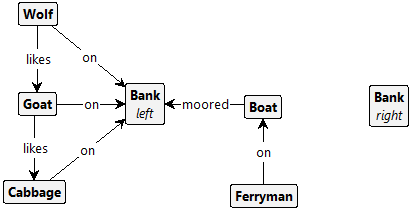
\includegraphics{images/groove_ferryman_start}
\caption{GROOVE grammar of the initial state of the ferryman model}\label{fig:groove_ferryman_start}
\end{figure}
\begin{figure}[h]
\centering
    \begin{subfigure}[b]{0.3\textwidth}
    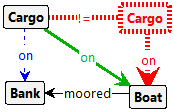
\includegraphics{images/groove_ferryman_rule_load}
    \caption{transition: load}
    \label{fig:groove_ferryman_load}
    \end{subfigure}
    ~
    \begin{subfigure}[b]{0.3\textwidth}
    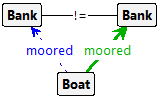
\includegraphics{images/groove_ferryman_rule_cross}
    \caption{transition: cross}
    \label{fig:groove_ferryman_cross}
    \end{subfigure}
    ~
    \begin{subfigure}[b]{0.3\textwidth}
    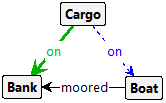
\includegraphics{images/groove_ferryman_rule_unload}
    \caption{transition: unload}
    \label{fig:groove_ferryman_unload}
    \end{subfigure}
\caption{GROOVE grammars for state-transitions of the ferryman model. The \texttt{Cargo} and \texttt{Bank} nodes are types: they indicate any cargo or river bank, respectively, that is selected with the state-transition. After the state-transition is complete, edges with a dashed blue line are removed and those with a solid green line are created. The red node and edge means: "if \texttt{Boat} has no other \texttt{Cargo} on it."}\label{fig:groove_ferryman}
\end{figure}
\par The state space generated from this model is seen in \cref{fig:groove_ferryman_statespace}. This state space contains 35 states and 70 transitions and is excellent for analysing state-transitions needed to get to a specific state. However, if one wants to visualize and animate the state-transitions that result in a specific state, these space generations tools don't have much to offer. GreenMirror can visualize this relatively easy. 
\begin{figure}[h]
	\centering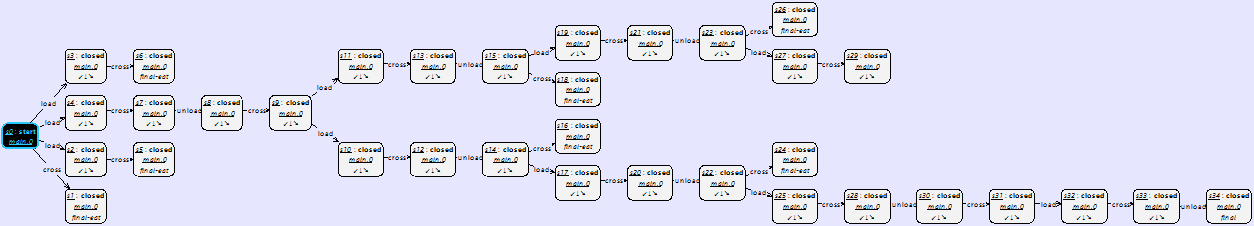
\includegraphics[width=\textwidth]{images/groove_ferryman_statespace}
    \caption{GROOVE generated state space of the ferryman model, using the breadth-first exploration strategy and final states acceptor, visualized using the compact tree layout and spanning tree filter. The blocks are the unique states and the labelled lines between them are the state-transitions. Note: because of the size of the image, the states and state-transitions are practically unreadable. This does not make the image any less relevant: it's an illustration of how a state space can become unclear easily and how it can be used to for analysis.}
    \label{fig:groove_ferryman_statespace}
\end{figure}
\par This model can be translated easily into files that can be interpreted by GreenMirror. For this example, the Groovy script model initializer and file trace selector implementations will be used (see \cref{sec:design;sub:interface}). \Cref{lst:greenmirror_ferryman_model} shows how the model is initialized. On line 1, the visualizer is initialized with a width of 500 pixels, a height of 300 pixels and a default JavaFX transition duration of 1000 milliseconds. On lines 3 to 46, the initial state is defined: the background, the ferry, the wolf, the goat and the cabbage nodes and all relations between them are created. These lines are roughly equivalent to \cref{fig:groove_ferryman_start}, with additional visualization information. Lines 49 to 58 are equivalent to \cref{fig:groove_ferryman_load}. A clear difference lies in the conditional that the ferry can not already hold a cargo node: GROOVE simply does not explore the states resulting from that state-transition, whereas GreenMirror gives an exception and aborts when this state-transition is erroneously encountered on a trace. Lines 61 to 68 and 71 to 80 are equivalent to respectively \cref{fig:groove_ferryman_cross,fig:groove_ferryman_unload}.
\lstinputlisting[label={lst:greenmirror_ferryman_model}, caption={example Groovy code for the ferryman model}]{code/ferryman.java}
\par The trace chosen for this example is the shortest trace that leads to the successful solution of the ferryman puzzle. In \cref{fig:groove_ferryman_statespace}, it is the path starting from the initial state, shown left in the figure, and ending in the state, shown in the bottom right corner of the figure. All other final states are unsuccessful solutions where either the goat or the cabbage gets eaten, or states that transition back into one of the displayed unique states. The trace is shown in \cref{lst:greenmirror_ferryman_trace}.
\lstinputlisting[label={lst:greenmirror_ferryman_trace}, caption={example trace for the ferryman model}]{code/ferryman.trace.txt}
\begin{wrapfigure}{o}{0.4\textwidth}\vspace{-22pt}
  \begin{center}
    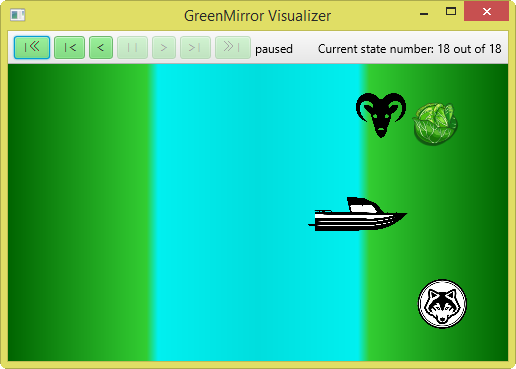
\includegraphics[width=0.38\textwidth]{images/greenmirror_ferryman}
  \end{center}
  \vspace{-10pt}\caption{a screenshot of the by GreenMirror visualized final state of the ferryman model as defined in \cref{lst:greenmirror_ferryman_model,lst:greenmirror_ferryman_trace}}\vspace{-20pt}
  \label{fig:greenmirror_ferryman}
\end{wrapfigure}
\par The ferryman model and trace from respectively \cref{lst:greenmirror_ferryman_model,lst:greenmirror_ferryman_trace} result in the GreenMirror visualization of which the final state is shown in \cref{fig:greenmirror_ferryman}. With just 80 lines of code and a pre-defined trace, the ferryman model of \cref{fig:groove_ferryman_start,fig:groove_ferryman,fig:groove_ferryman_statespace} can be visualized and animated in GreenMirror for further analysis. It took GreenMirror about one second to interpret the model and the trace, followed by roughly five seconds to add all data to the visualizer after which the user could start moving through the model states. As is seen from the code in \cref{lst:greenmirror_ferryman_model}, images, geometric shapes such as rectangles and directed relations can be used. Furthermore, nodes can be placed according to their relations and complex (programming) logic can be added. \Cref{sec:features} contains more information about the currently available features.
\newpage
%--------------------------------------------------------------------------------
%----------------------------------------------------------------------
\section{Features}\label{sec:features}
Knowledge of the features of GreenMirror is imperative when using the application. The two parts GreenMirror is composed of and their usage is first described in \cref{sec:features;sub:clientserver}. The way a model is interpreted is then elaborated upon in \cref{sec:features;sub:nodrel}, followed by a description of an integral part of the visualizations in \cref{sec:features;sub:placement}: node placement. Further possibilities are presented by discussing all currently available commands in \cref{sec:features;sub:commands}. \Cref{sec:features;sub:log,sec:features;sub:gridbuilder} briefly expand upon two auxiliary functionalities: the log and the \lstinline{GridBuilder} class, respectively.
%--------------------------------------------------------------------------------
\subsection{Client and server}\label{sec:features;sub:clientserver}
The GreenMirror application is divided into two distinct components: the client and the server. The client interprets the user's model and translates it into commands. The server performs the actual visualization on the basis of these commands. Due to this decoupling, the framework is more maintainable and extensible and can thus be easily linked to other components or component versions.
\par Both components have to be executed using command line options. For the client to run, it needs a server to be available. To start the server, only one option has to be provided: the port. Use, for example, the option \lstinline{--port=81} to run the server on port 81. The \lstinline{--verbose} option can be added to enable verbose output to the log and \lstinline{--help} to show all available command line options.
\par The client has three required options: \lstinline{--host}, \lstinline{--model} and \lstinline{--trace}. If a GreenMirror server is running local on port 81, the first option would look like \lstinline{--host=127.0.0.1:81}. To initialize a model using a Groovy script (which is currently the only supported model initializer), use \lstinline{--model=groovyscript:<groovyfile>} and to select a trace using the file selector (which is currently the only supported trace selector), use \lstinline{--trace=file:<tracefile>}. \lstinline{<*file>} should, of course, be replaced with the corresponding file names. Similar to the server, \lstinline{--verbose} and \lstinline{--help} can also be used with the client. For more details, see \cref{sec:design;sub:generalwf,sec:design;sub:detailedwf,sec:design;sub:interface}.
%--------------------------------------------------------------------------------
\subsection{Nodes and relations}\label{sec:features;sub:nodrel}
Tools such as GROOVE \cite{rensink2004} use \emph{nodes} and \emph{edges} to define their model. This terminology can not simply be copied, because the definition and usage of an edge is slightly different than the equivalent entity used in GreenMirror. GreenMirror uses \emph{nodes} and directional \emph{relations} to define the model. State-transitions consist of adding and removing nodes, altering the appearance of nodes and changing relations between nodes. \\
Node properties include a type, a name, labels and an appearance wrapper, all of which are optional. When the node is added to the model, it receives an internal identification number; "ID" for short. The user does not have to interact with this ID in any way. Nodes also store their relations with other nodes. \\
Relations are always directional, going from "node A" to "node B". All relations have a name, a placement, a rigidity and a temporary appearance for node A, of which the latter lasts for the duration of the relation. These properties are optional, although it is recommended to always specify a name. There are two kinds of relations: placement relations, indicating that node A has a placement relative to node B on the visualizer, and non-placement relations, where the placement is set to \lstinline{NONE}. The rigidity property can only be set for placement relations. When set to true it indicates that node A should follow when node B moves on the visualizer. If the rigidity is set to false, the placement is only calculated and applied when the relation is created: it won't be maintained when node B moves.
\par Each GreenMirror node that has a visual appearance needs to store and track the properties of its FX. This is internally done using implementations of the abstract \lstinline{FxWrapper} class. The FX type can only be defined once for every GreenMirror node. The currently supported FX types are:
\begin{itemize}
\item rectangle;
\item circle;
\item text; and
\item image (with a local or remote source).
\end{itemize}
\par Per FX type, certain properties can be set only initially and some can also be set or changed after the node's FX initialization. Due to the nature of GreenMirror, all properties of the latter type must be animatable. The \texttt{opacity} property, for example, is animatable by default by the JavaFX library. The \texttt{width} of a rectangle, on the other hand, is not animatable by default. GreenMirror includes animation support for some properties such as \texttt{width} so these properties can be changed during state-transitions. GreenMirror also supports the animation of some discrete properties, such as the \texttt{text} property of the text FX type. This is done by using a fast fade-out on the JavaFX node, changing the property and then using a fast fade-in. Support for additional FX types and FX type properties can be easily added to the framework. See \cref{sec:design;sub:fxwrapper,app:ext;sub:fxwrapper,app:ext;sub:fxpropertywrapper}.
%--------------------------------------------------------------------------------
\subsection{Node placement}\label{sec:features;sub:placement}
Placements are an important aspect of the visualization of nodes and their relations. They provide a level of abstraction and let the user worry rather about the model than about the actual coordinates of nodes on the visualizer. Placement relations between nodes indicate that one node of the relation, node A, is placed in a specific respect to the other node of the relation, node B. There are currently several extensions of the abstract \lstinline{Placement} class implemented which are described below and are illustrated in \cref{fig:placements}. Every instance of \lstinline{Placement} also has an optional position relative to the placement. For example: if a node A has an edge top placement with relative position \lstinline{(0, -20)} on node B, node A is placed 20 pixels above (and centred on) the edge of node B.
\begin{description}
\item[\texttt{Corner*Placement}] A placement on any of the corners of a JavaFX node: top left, top right, bottom right or bottom left.
\item[\texttt{Edge*Placement}]  A centred placement on any of the edges of a JavaFX node: top, right, bottom or left.
\item[\texttt{MiddlePlacement}] A placement in the exact middle of a JavaFX node.
\item[\texttt{EdgePlacement}]   A placement on the edge of a JavaFX node, according to a specified angle. An angle of zero degrees is the equivalent an edge top placement, and an angle of 90 degrees (positive) is the equivalent of an edge right placement. 
\item[\texttt{CustomPlacement}] A placement where only the relative position data is used to determine the coordinates. The relative position data is relative to the coordinates calculated for the \lstinline{MiddlePlacement}.
\item[\texttt{RandomPlacement}] A random placement on a JavaFX node. Upon receiving this placement data, the server replaces this with a \lstinline{CustomPlacement} where the relative position is set to the calculated, relative coordinates of the \lstinline{RandomPlacement}. This is done so the random coordinates aren't recalculated every time node B moves (in the case of a rigid placement relation).
\item[\texttt{NoPlacement}] The default for a relation.
\end{description}
\begin{figure}[h]
  \centering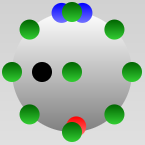
\includegraphics{images/placements}
  \caption{an example available placements on a circle FX node. The green circles have a corner* (or at least, what would have been the corner), edge* or middle placement, the blue ones an edge placement with -10 and 10 degrees, the black one a custom placement with relative position \lstinline{(-10, 0)} and the red one a random placement.}
  \label{fig:placements}
\end{figure}
%--------------------------------------------------------------------------------
\subsection{Commands}\label{sec:features;sub:commands}
In the current version of GreenMirror, communication between the client and the server is one way: all supported commands are meant to be sent from the client to the server. With the information in this section and \cref{sec:design;sub:interchange}, one can develop a completely new client or server that can work with the current version of GreenMirror. For a better overview, the commands have been divided into \cref{tab:commands_vis,tab:commands_model}: the first is about commands relating to the visualizer and the handling of state-transitions, the second is about changes in the model. In the tables, the command name is in the upper left corner, the parameters, their type and their description on the right and the command description underneath those. This section is meant to give an overview of the currently available commands used within GreenMirror: it is not as detailed as the JavaDoc documentation that is available on the repository of this project.
\begin{longtable}{ |l|l r| }
\caption{commands pertaining to the visualizer and the handling of state-transitions}\label{tab:commands_vis}
\\ \hline \multirow{2}{*}{\textbf{Initialization}}
   & \texttt{width} & integer 
\\ & \multicolumn{2}{|l|}{The width of the visualizer window.} 
\\ \cline{2-3} & \texttt{height} & integer
\\ & \multicolumn{2}{|l|}{The height of the visualizer window.}
\\ \cline{2-3} & \texttt{defaultAnimationDuration} & double
\\ & \multicolumn{2}{|l|}{The default time animations will take to complete.}
\\ \cline{2-3} & \texttt{rotateRigidlyRelatedNodesRigidly} & boolean
\\ & \multicolumn{2}{|l|}{\parbox[t]{10.3cm}{Whether the "A" node of a rigid relation should rotate rigidly when the "B" node is rotated.\Bstrut}}
\\ \cline{2-3} \multicolumn{3}{|l|}{\parbox[t]{14.1cm}{\vspace{5px}The initialization command initializes and opens the visualizer with the passed parameters. This should come \emph{before} any command pertaining to the model.\vspace{10px}}}
%--------------------
\\ \hline \pagebreak \hline \multirow{2}{*}{\textbf{SetAnimationDuration}}
   & \texttt{duration} & double
\\\nopagebreak[4] & \multicolumn{2}{|l|}{The duration of all following animations, in milliseconds.}
\\\nopagebreak[4] \cline{2-3} \multicolumn{3}{|l|}{\parbox[t]{14.1cm}{\vspace{5px}This sets the duration of all atomic animations. For example: if the animation duration is set to 1000 milliseconds and five animations will be played sequentially, the total animation duration is 5000 milliseconds.\vspace{10px}}}
%--------------------
\\ \hline\hline \multirow{2}{*}{\textbf{Flush}}
   & \texttt{delay} & double
\\ & \multicolumn{2}{|l|}{The delay that is added after the previous animation, in milliseconds.}
\\ \cline{2-3} \multicolumn{3}{|l|}{\parbox[t]{14.1cm}{\vspace{5px}By default, all animations resulting from one state-transition are played parallel to each other. This command creates a new queue: the set of parallel animations created after this command are played after the set of previously created animations. Optionally, a delay can be added between the previous and upcoming set of animations. Also see \cref{sec:design;sub:states}. \vspace{10px}}}
%--------------------
\\ \hline\hline \multicolumn{3}{|l|}{\multirow{2}{*}{\textbf{EndTransition}}}
\\ \multicolumn{3}{|l|}{\parbox[t]{14.1cm}{\vspace{5px} This command signals the server that the state-transition has ended. \vspace{10px}}}
%--------------------
\\ \hline\hline \multicolumn{3}{|l|}{\multirow{2}{*}{\textbf{StartVisualization}}}
\\ \multicolumn{3}{|l|}{\parbox[t]{14.1cm}{\vspace{5px} The command that tells the server that the visualizations may start. The current version of this server handles this by transitioning to the first state. \vspace{10px}}}
%--------------------
\\ \hline\hline \multicolumn{3}{|l|}{\multirow{2}{*}{\textbf{ExitVisualizer}}}
\\ \multicolumn{3}{|l|}{\parbox[t]{14.1cm}{\vspace{5px} This command communicates to the server that the visualizer should exit. In this version of GreenMirror, the client sends this command if a fatal error is encountered in the user's model. \vspace{10px}}}
\\\hline\end{longtable}
%-*-*-*-*-*-**-*--*-*--*-**--**-*--**-*-*-*--**-*--*
\begin{longtable}{ |l|l r| }
\caption{commands pertaining to the user's model}\label{tab:commands_model}
%--------------------
\\\hline \multirow{2}{*}{\textbf{AddNode}}
   & \texttt{id} & integer 
\\ & \multicolumn{2}{|l|}{The unique, internal ID of the GreenMirror node.} 
\\ \cline{2-3} & \texttt{identifier} & string
\\ & \multicolumn{2}{|l|}{The identifier of the GreenMirror node: the user-defined type and name.}
\\ \cline{2-3} \multicolumn{3}{|l|}{\parbox[t]{14.1cm}{\vspace{5px} This signals that a node has been added to the user's model. The visualizer doesn't have to do anything yet: the FX is yet to be defined at this point. \vspace{10px}}}
%--------------------
\\ \hline\hline \multirow{2}{*}{\textbf{AddRelation}}
   & \texttt{name} & string 
\\ & \multicolumn{2}{|l|}{The name of the relation.} 
\\ \cline{2-3} & \texttt{nodeA} & integer
\\ & \multicolumn{2}{|l|}{The internal ID of node A.}
\\ \cline{2-3} & \texttt{nodeB} & integer
\\ & \multicolumn{2}{|l|}{The internal ID of node B.}
\\ \cline{2-3} & \texttt{placement} & string
\\ & \multicolumn{2}{|l|}{The placement data of node A on node B.}
\\ \cline{2-3} & \texttt{rigid} & boolean
\\ & \multicolumn{2}{|l|}{Whether the relation is rigid or not.}
\\ \cline{2-3} & \texttt{tempFX} & FxWrapper
\\ & \multicolumn{2}{|l|}{The temporary FX of node A.}
\\ \cline{2-3} \multicolumn{3}{|l|}{\parbox[t]{14.1cm}{\vspace{5px} This indicates that a relation has been added between a node "A" and a node "B". If \texttt{placement} is set, the server should handle this. The same goes for \texttt{tempFX}. \vspace{10px}}}
%--------------------
\\ \hline\hline \multirow{2}{*}{\textbf{RemoveNode}}
   & \texttt{id} & integer 
\\ & \multicolumn{2}{|l|}{The internal node ID.} 
\\ \cline{2-3} \multicolumn{3}{|l|}{\parbox[t]{14.1cm}{\vspace{5px} This commands signals that a GreenMirror node has been removed from the user's model. Consequently, all relations have also been removed. \vspace{10px}}}
%--------------------
\\ \hline\hline \multirow{2}{*}{\textbf{RemoveRelation}}
   & \texttt{id} & string
\\ & \multicolumn{2}{|l|}{The unique ID of the relation.} 
\\ \cline{2-3} & \texttt{nodeA} & integer
\\ & \multicolumn{2}{|l|}{The internal ID of node A.} 
\\ \cline{2-3} \multicolumn{3}{|p{14.1cm}|}{\vspace{5px} This commands signals that a relation has been removed. The server should also handle restoring the FX of node A in the case a temporary FX was set. \vspace{10px}}
%--------------------
\\ \hline\hline \multirow{2}{*}{\textbf{SetNodeFX}}
   & \texttt{id} & integer
\\ & \multicolumn{2}{|l|}{The internal ID of the GreenMirror node.} 
\\ \cline{2-3} & \texttt{fx} & FxWrapper
\\ & \multicolumn{2}{|l|}{The FX values.} 
\\ \cline{2-3} \multicolumn{3}{|p{14.1cm}|}{\vspace{5px}This commands communicates with what properties and values the FX of a node should be set. The \texttt{fx} parameter can include all properties that can be set, initially or otherwise (see \cref{sec:features;sub:nodrel}).\vspace{10px}}
%--------------------
\\ \hline\hline \multirow{2}{*}{\textbf{ChangeNodeFX}}
   & \texttt{id} & integer
\\ & \multicolumn{2}{|l|}{The internal ID of the GreenMirror node.} 
\\ \cline{2-3} & \texttt{fx} & FxWrapper
\\ & \multicolumn{2}{|l|}{The new FX values.} 
\\ \cline{2-3} \multicolumn{3}{|p{14.1cm}|}{\vspace{5px} This commands indicates that the FX of a GreenMirror node has been changed. The \texttt{fx} parameter can include only animatable properties (see \cref{sec:features;sub:nodrel}). \vspace{10px}}
\\\hline\end{longtable}
%--------------------------------------------------------------------------------
\subsection{Log}\label{sec:features;sub:log}
It is assumed that any stakeholder working with the tool wants as much data and information as possible about what is happening. GreenMirror uses a static \lstinline{Log} class that accepts any implementation of \lstinline{PrintStream}. During runtime both the client and the server send data and information to their respective log sinks. A time stamp that is accurate to the millisecond is included with each entry, so performance can also be analysed. The client uses \lstinline{System.out} as its log sink, seeing as it does not have a graphical user interface. The server uses \lstinline{System.out} and, as it does have a graphical user interface, GreenMirror's \lstinline{WindowLogger} implementation (depicted in \cref{fig:log}). As was briefly mentioned in \cref{sec:features;sub:clientserver}, a verbose option can be enabled which results in the log being filled with more raw data.
\begin{figure}[h]
  \centering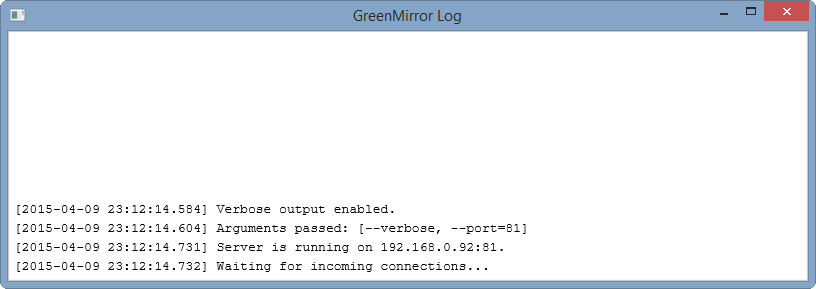
\includegraphics[width=0.95\textwidth]{images/log}
  \caption{an instance of \lstinline{WindowLogger} right after the server has been executed}
  \label{fig:log}
\end{figure}
%--------------------------------------------------------------------------------
\subsection{The \texttt{GridBuilder} class}\label{sec:features;sub:gridbuilder}
\begin{wrapfigure}{o}{0.25\textwidth}\vspace{-22pt}
  \begin{center}
    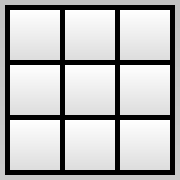
\includegraphics[width=0.23\textwidth]{images/grid}
  \end{center}
  \vspace{-10pt}\caption{the result of the \lstinline{GridBuilder} example code of \cref{lst:gridbuilder}}\vspace{-20pt}
  \label{fig:grid}
\end{wrapfigure}
GreenMirror has an auxiliary \lstinline{GridBuilder} class created to take away the tedious work of building a grid of nodes. It supports properties such as the amount of cells, the cell width and height, cell spacing, cell colour, borders, a background colour and the type and name prefix for every GreenMirror node it creates. It builds the grid by creating one GreenMirror node per cell and one for the background, all of which have the rectangle FX type. \Cref{lst:gridbuilder} shows an example of how short the code is to create a TicTacToe grid, in contrast to defining every single GreenMirror node, not to mention the tedious work of getting their exact positioning right. Doing the same without the \lstinline{GridBuilder} class takes roughly 30 lines of sloppy code. The result of \cref{lst:gridbuilder} is visible in \cref{fig:grid}.
\begin{lstlisting}[label={lst:gridbuilder}, caption={example code the user can use to build a grid of nodes}]
new GridBuilder("ticTacToeGrid:cell_")
    .setCellCount(3, 3)
    .setCellSize(50, 50)
    .setCellFill("linear-gradient(to bottom, #FFF, #DDD)")
    .setCellSpacing(5)
    .setBorderSize(5) // top, right, bottom and left
    .setBackgroundFill("black")
    .build(10, 10) // Coordinates on the visualizer
    .getNodes()
\end{lstlisting}
\newpage
%--------------------------------------------------------------------------------
%----------------------------------------------------------------------
\section{Design and implementation}\label{sec:design}
This section gives more detailed information about the design of GreenMirror and some details of its implementation. GreenMirror is written with version 8 of the Java Runtime Environment and developed under Eclipse Luna. It highly depends on the integrated JavaFX library and uses JUnit \cite{junit} for testing, JOpt Simple \cite{joptsimple} for handling the command line options (see \cref{sec:design;sub:detailedwf}), Groovy \cite{groovy} (see \cref{sec:design;sub:interface}) for its JSON implementation and scripting capabilities and the Eclipse JDT annotation package for using \lstinline{NonNull} annotations. GreenMirror is composed of 114 classes in 12 packages, which sums up to a total of 7429 lines of code.
%--------------------------------------------------------------------------------
\subsection{Package structure}\label{sec:design;sub:package}
GreenMirror's package structure is fairly self-evident. Still, a short explanation per package is in place. Details about how to extend certain subpackages are available in \cref{app:ext}. Corresponding class diagrams depicting all relations between the classes are unfortunately too large to be a useful addition to this report, although they are available on the repository.
\begin{description}
\item[\texttt{greenmirror}] is the main package containing classes shared by the client and server.
\item[\texttt{greenmirror.client}] contains all classes that pertain solely to the client.
\item[\texttt{greenmirror.client.modelinitializers}] contains all implemented model initializers that can be used by the client. See \cref{sec:design;sub:interface}.
\item[\texttt{greenmirror.client.traceselectors}] contains all implemented trace selectors that can be used by the client. See \cref{sec:design;sub:interface}.
\item[\texttt{greenmirror.commandlineoptionhandlers}] contains all command line option handlers, both for the client and the server. The \lstinline{@ClientSide} and \lstinline{@ServerSide} annotations indicate where they are used. See \cref{sec:design;sub:detailedwf}.
\item[\texttt{greenmirror.commands}] contains all commands that are sent from the client to the server and vice versa. It also contains all handlers that interpret and handle received commands. The handlers have \lstinline{@ClientSide} and \lstinline{@ServerSide} annotations to indicate where their respective commands are received.
\item[\texttt{greenmirror.fxpropertywrappers}] contains all implemented wrappers for FX properties. See \cref{sec:design;sub:fxwrapper}.
\item[\texttt{greenmirror.fxwrappers}] contains all implemented FX wrappers. See \cref{sec:features;sub:nodrel,sec:design;sub:fxwrapper}.
\item[\texttt{greenmirror.placements}] contains all implemented placements. See \cref{sec:features;sub:placement}.
\item[\texttt{greenmirror.server}] contains all classes that pertain solely to the server.
\item[\texttt{greenmirror.server.playbackstates}] contains the playback states of the visualizer. See \cref{sec:design;sub:patterns}.
\item[\texttt{greenmirror.tests}] contains several unit tests to validate the workings of GreenMirror. See \cref{sec:validation}.
\end{description} 
%--------------------------------------------------------------------------------
\subsection{General work-flow}\label{sec:design;sub:generalwf}
\begin{figure}[h]
  \centering
  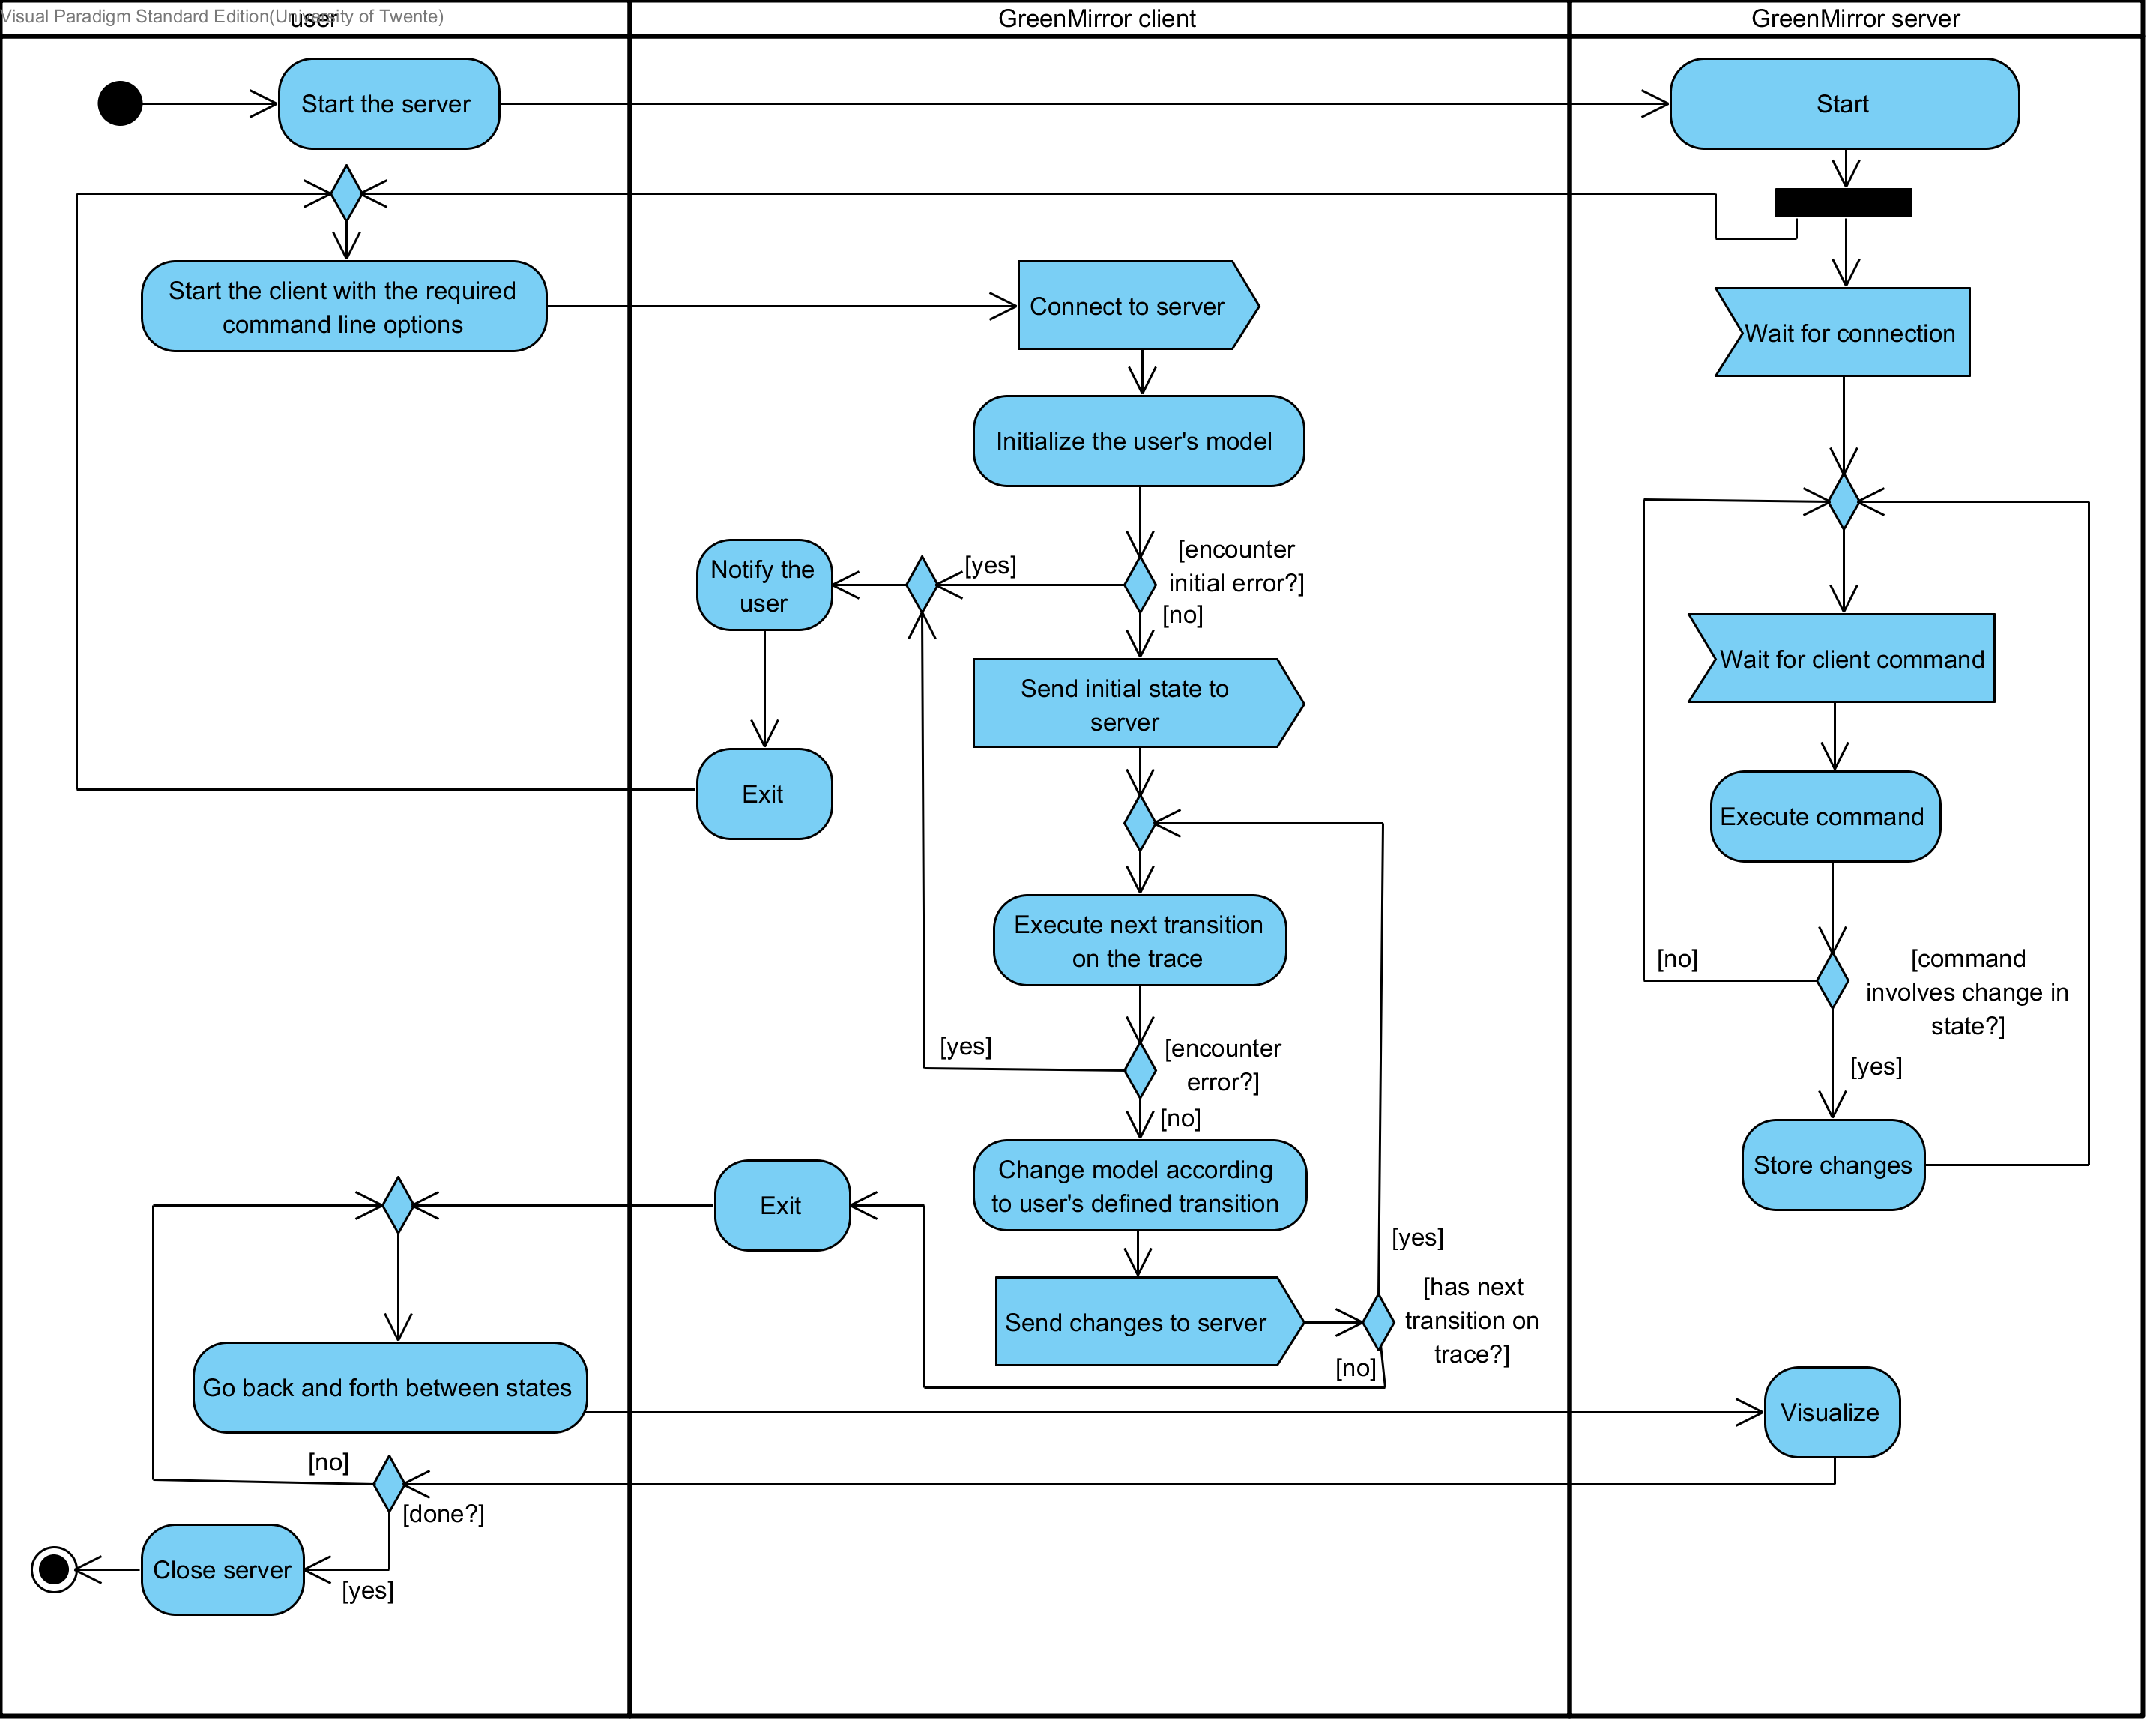
\includegraphics[width=1.0\textwidth]{diagrams/AD_generalworkflow}
  \caption{simplified activity diagram of the general work-flow}\label{fig:ad_generalworkflow}
\end{figure}
The general work-flow of a typical execution of the application is illustrated in the simplified activity diagram of \cref{fig:ad_generalworkflow}. This is meant to be fairly general: the exact work-flow depends on the used model initializers, the used trace selector and the user's model. In the current version, the visualization can only start when the whole model has been interpreted by the client and has been sent to the server. This behaviour is meant to ensure top performance while transitioning through the states, but can be easily modified.
%--------------------------------------------------------------------------------
\subsection{Detailed work-flow}\label{sec:design;sub:detailedwf}
The first thing that occurs when operating the application is starting up the client or server and parsing the command line options. GreenMirror uses the JOpt Simple library \cite{joptsimple} to parse command line options in the same way options can be used with executables of *nix operating systems. Available command line options implement the \lstinline{CommandLineOptionHandler} interface. This contains everything needed to handle options: option and argument specification, processing order, argument validation and option processing. See \cref{fig:sd_generalstartup} (\cref{app:seq}) for the (simplified) sequence of these events. From the diagram can be seen that the options are all validated before they are processed. This prevents partial processing without having all required and valid options (for example: initializing the model without a valid server address).\\
The importance of the validating, parsing and processing of command line options, however, should be explicitly stated. The complete set of the application's functions work as a direct consequence of the processing of these options. For example: the handler for the \lstinline{--host} option handles establishing the connection to the server and the handler for the \lstinline{--trace} option executes the trace. This results in the fact that new functionalities that should be executed during start-up can be easily added by implementing and adding new option handlers (see \cref{app:ext} for instructions).
\par\begin{wrapfigure}{r}{0.38\textwidth}\vspace{-20pt}
  \begin{center}
    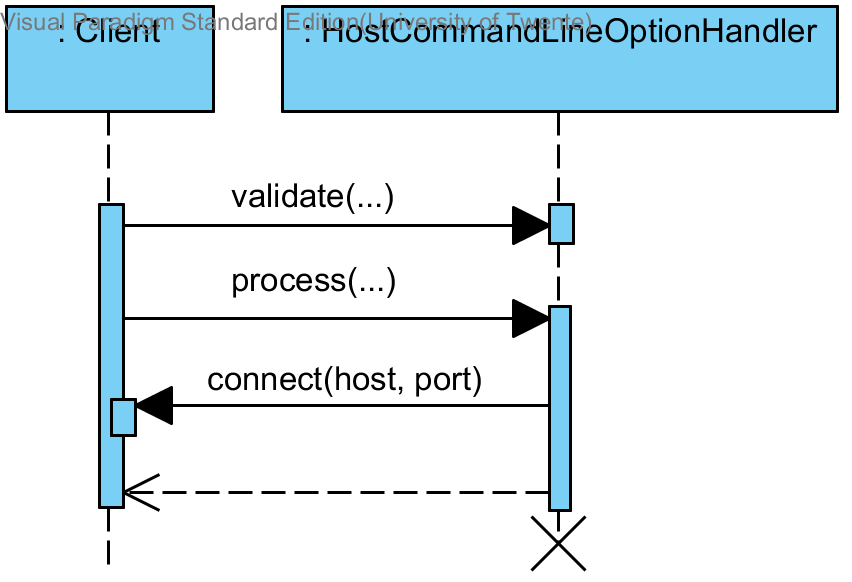
\includegraphics[width=0.36\textwidth]{diagrams/SD_client_host}
  \end{center}
  \vspace{-20pt}\caption{simplified sequence diagram of the handling of the \lstinline{--host} command line option}\vspace{-15pt}
  \label{fig:sd_client_host}
\end{wrapfigure}
Next are the implemented command line option handlers of the client. From here on out, the assumption is made that all required options are passed (\lstinline{--host}, \lstinline{--model} and \lstinline{--trace}) and that their arguments are valid. If that would not be the case, GreenMirror would have observed this before processing and would have notified the user before terminating, as is described in the previous paragraph. The first option that will be processed is the \lstinline{--host} option, which connects to the server. This is very straightforward and will requires no further elaboration. See \cref{fig:sd_client_host}.
\par Handling the model initializer option \lstinline{--model} is far more interesting. Several notable things are worth stating when looking at the sequence diagram in \cref{fig:sd_client_model} (\cref{app:seq}). Firstly, it can be seen that multiple model initializers can be selected. This is designed this way so the user can define the model in more than one way, perhaps even with the use of modules. In practise this can be used by simply passing the \lstinline{--model} option multiple times. Multiple model initializers are executed in the same order as they were passed via the command line. Secondly, a model initializer should define the model with the initial state and the state-transitions. The initial state can be defined by defining the initial nodes and relations and adding them to the controller. This sends the information directly to the server. Each state-transition is defined as an instance of the \lstinline{ModelTransition} class and holds a \lstinline{groovy.lang.Closure} field. This is code that is executed when the transition is executed and should transition the model to the next state. How the model initializer exactly defines the initial state and the state-transitions is up to the implementation (see \cref{sec:design;sub:interface}). Finally, when the model initializers have been executed and thus the initial state has been defined, GreenMirror sends the \lstinline{StartVisualization} command to the server, indicating that the transition to the first state can be performed. 
\par The \lstinline{--trace} option is handled next. See \cref{fig:sd_client_trace} (\cref{app:seq}) for the sequence diagram. This follows somewhat the same structure as the model initializer option handler, with a few slight differences. Only one \lstinline{TraceSelector} can be used. However, multiple \lstinline{ModelTransition}s can be executed with each transition from the trace, due to the fact that the \lstinline{ModelTransition} instance has a regular expression pattern that matches with zero to unlimited transitions from the trace. These transitions are executed in the order in which the model initializer added them to the controller. After each executed transition, GreenMirror sends an \lstinline{EndTransition} command to the server, indicating that a new state has been reached. If the user wants GreenMirror to refrain from sending this command, perhaps because the executed transition is part of the next one, the \lstinline{supplemental} flag of the \lstinline{ModelInitializer} instance can be set to \lstinline{true}.
\begin{figure}[ht]
  \centering
  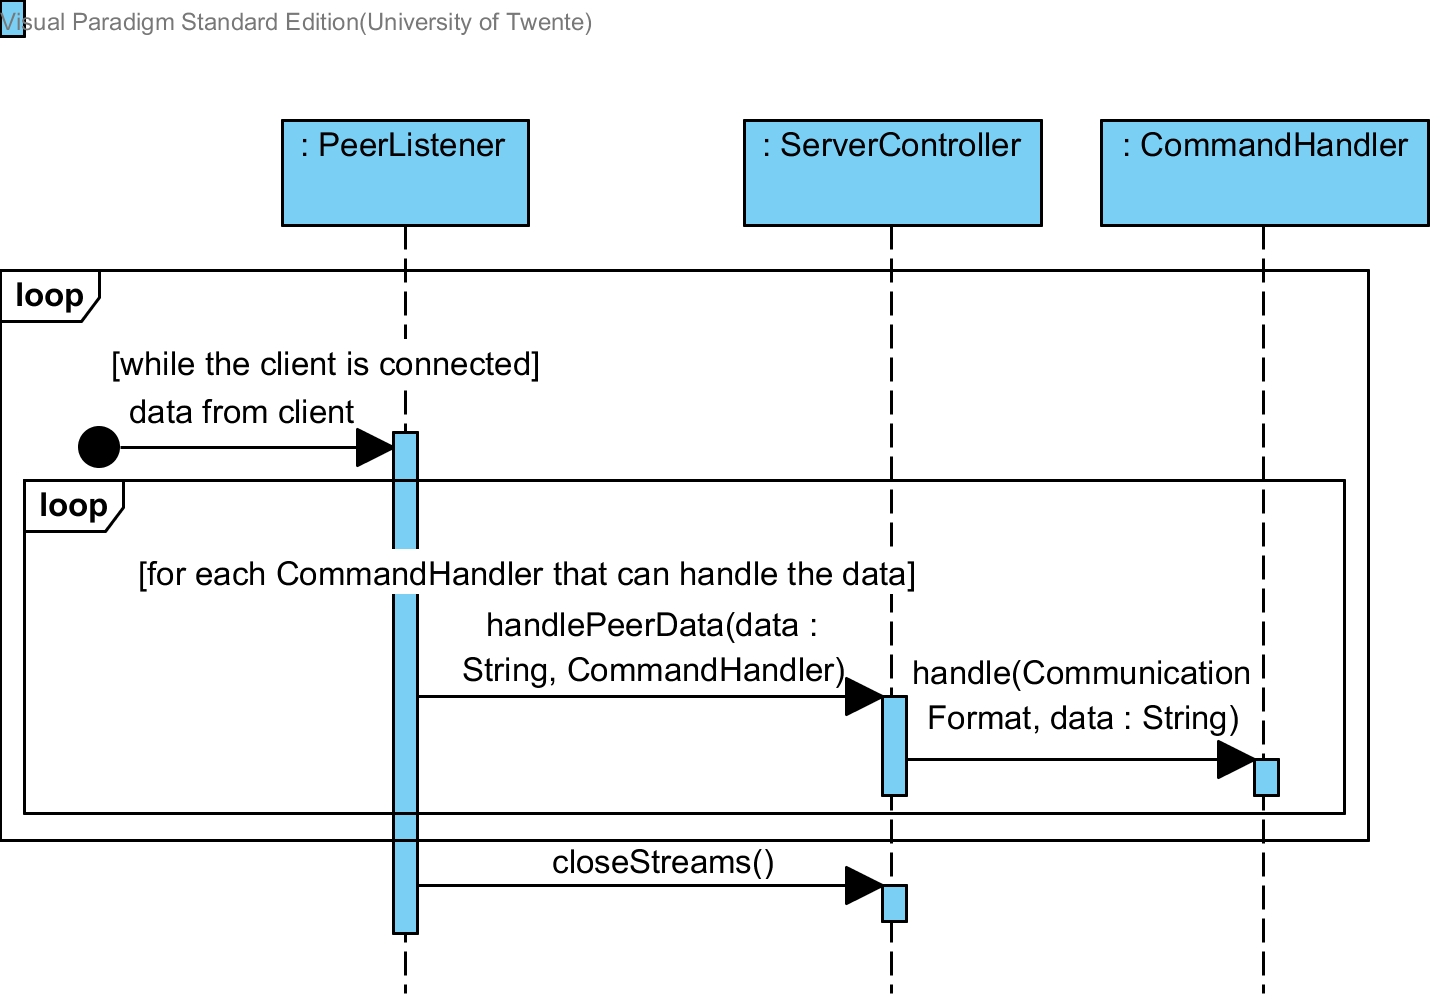
\includegraphics[width=0.6\textwidth]{diagrams/SD_server_receivecommand}
  \caption{simplified sequence diagram of the server receiving data}\label{fig:sd_server_receivecommand}
\end{figure}
\par The client is now finished and will close. In the meanwhile, the server has received the commands the client has sent. Every command is passed to the correct \lstinline{CommandHandler} in the sequence as shown in \cref{fig:sd_server_receivecommand}. What exactly happens in the \lstinline{handle(CommunicationFormat, String)} method of the \lstinline{CommandHandler} entirely depends on the received command.
\par After the client has sent the \lstinline{StartVisualization} command, the server starts the transition to the first state. Upon finishing, the correct toolbar buttons are enabled and the user can start interacting with the visualizer. What is seen in the sequence diagram of the user interaction (\cref{fig:sd_server_userinteraction} in \cref{app:seq}) is that all visualization parameters of the state-transition are derived from the button the user clicked on.
%More on this will be explained in \cref{subsec:implementationdetails}.
%TODO: check if the line above should be used (and the line above that).
%--------------------------------------------------------------------------------
\subsection{Interface design}\label{sec:design;sub:interface}
This section discusses the available interfaces for tool owners that provide ways of loading models into GreenMirror, and the current implementations. Loading a model consists of two parts: defining the model and providing the trace that defines in which order state-transitions will take place. Both parts have corresponding interfaces: respectively \lstinline{ModelInitializer} and \lstinline{TraceSelector}.
\par The model initializer has a few responsibilities. First and foremost it must, in the most general sense and not surprisingly, initialize the model according to the specifications of the user. More specifically: it must receive information from the user about how the initial state of the model is defined and how different state-transitions influence the model and the visualization. How the model initializer receives or retrieves this information is up to the implementation. Once it has received this information, it can add nodes to the client controller, remove nodes, add relations, etcetera. These changes are automatically conveyed to the server. The model initializer can also use the interface with the controller to send commands directly to the server, by use of the currently available commands in the \lstinline{greenmirror.commands} package. This behaviour is, however, not recommended, because this circumvents the logic incorporated in updating the model via the controller. It is meant to provide the possibility to send auxiliary commands such as the \lstinline{SetAnimationDuration} command.
\par The model initializers must define which state-transitions can happen by adding new instances of \lstinline{ModelTransition} to the controller. As mentioned in \cref{sec:design;sub:detailedwf}, this class has a \lstinline{groovy.lang.Closure} field that changes the model when the closure is executed. This type is chosen to directly support the first implemented model initializer, although it is not restricted to this first implementation. The closure can accept arguments based on the transitions on the trace. This is best explained using an example. Suppose the user wants to visualize a ConnectFour game. It would be unwieldy to define a state-transition for every possible move (although there are only seven at the most), so the user defines one state-transition that uses the regular expression \lstinline{^move([0-6])\$} to accept transitions from a trace. This means it needs the number of the column as an argument in the closure that executes the state-transition. Fortunately, the Groovy library supports this and GreenMirror takes advantage of this by supporting string and integer type arguments.
\par The server could be completely re-purposed by implementing different commands and command handlers. However, if the server is used as a visualizer, the model initializer has the responsibility of making sure the server first receives the initialization command. Without it, there is no JavaFX stage to which JavaFX nodes can be added. A tool owner developing a new model initializer could choose to delegate this responsibility to the user.
\par The model initializer that has been implemented in this first version of GreenMirror is based on Groovy \cite{groovy}. Groovy is a dynamic language for the Java platform and provides a vast array of useful features. Specifically, the model initializer uses Groovy's script functionalities. This choice was made due to the following reasons.
\begin{enumerate}
\item The user receives the power and flexibility of a full-featured programming language, but still is easy to learn. This means that both advanced programmers and users without much experience can use it.
\item The user scripts can be executed during runtime, meaning that, while employing a complete programming language, the GreenMirror framework doesn't have to be recompiled every time the user alters his model.
\item A clear interface with the controller can be provided to the user, which Groovy calls a \emph{base class}. The user can refer in his script to the base class' methods without referring to any object. This works as if the user is programming in the context of one of the methods of the base class (which it also comes down to, internally).
\end{enumerate}
\Cref{lst:groovyexample} shows an example of a user script that can be executed by the Groovy script model initializer. \Cref{fig:groovyexample} shows a screenshot of its resulting visualization. It can be seen from the listing that chained statements are possible and actually encouraged to improve the readability of the script. Another notable advantage is that it is easily seen that calls to the base class (and thus indirectly to the controller) indicate a read from or a write to the model. For example, creating a new \lstinline{Node} instance does not mean it is added to the model: \lstinline{addNodes()} takes care of that.
\lstinputlisting[label={lst:groovyexample}, caption={example Groovy script defining the user's state-transition model}]{code/example.java}
\begin{figure}[H]
  \centering
  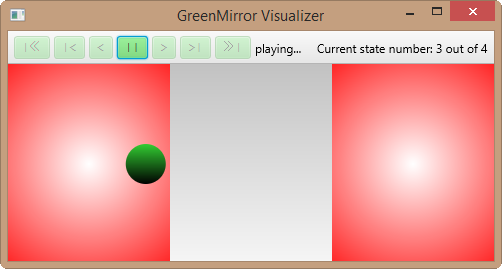
\includegraphics{images/groovyexample}
  \caption{a screenshot of the executing visualization of \cref{lst:groovyexample} with the trace from \cref{lst:traceexample}}\label{fig:groovyexample}
\end{figure}
\par After the model initializer has set the initial state and saved all \lstinline{ModelTransition}s, the selected \lstinline{TraceSelector} is executed. The current \lstinline{FileTraceSelector} implementation retrieves the trace from a text file where the transitions are separated by a newline. In the visualization example of \cref{fig:groovyexample}, the trace file looked like \cref{lst:traceexample}. In the toolbar of \cref{fig:groovyexample} a state count of four can be seen, while three transitions are in the trace. This is naturally because the initial state is included in the count.	
\begin{lstlisting}[label={lst:traceexample}, caption={example trace file for the model defined in \cref{lst:groovyexample}}]
switch
switch
switch
\end{lstlisting}
Both the \lstinline{ModelInitializer} and \lstinline{TraceSelector} interfaces accept one argument from the command line. This should be the source of the model and the trace, respectively. In \lstinline{GroovyScriptModelInitializer} it is the file name of the Groovy script, while in \lstinline{FileTraceSelector} it is the name of the file containing the trace. In future implementations that, for example, connect GreenMirror to another tool, this could be the name of the model.
%--------------------------------------------------------------------------------
\subsection{Implemented design patterns}\label{sec:design;sub:patterns}
GreenMirror conforms to several design patterns \cite{kuchana2004,sourcemaking} to stimulate future development and the overall maintainability of the framework. \Cref{tab:patterns} describes several implemented patterns, in alphabetical order. The name on the left side is the name of the design pattern. The right side describes the classes or structures that use the design pattern and contain information about the contexts in which the patterns are implemented.
\newpage\begin{longtable}{ |l p{10cm}| }
\caption{design patterns used in the GreenMirror framework}\label{tab:patterns}\\
\hline\multirow{2}{*}{\textbf{Builder}}
   & \texttt{GridBuilder} \\* & This class first accepts several required and optional parameters, after which it constructs the grid and finally returns the \texttt{NodeList} instance that contains the nodes that make up the grid. See \cref{sec:features;sub:gridbuilder} for more information and an example. \\
\hline\multirow{2}{*}{\textbf{Command}}
   & \texttt{Command} \\* & Whenever a subclass of \texttt{Command} is instantiated, the arguments are passed to its constructor. The \texttt{prepare()} method is called, in which the command can optionally execute preparations. Finally, the \texttt{getFormattedString(CommunicationFormat)} is called to retrieve a string that will be sent to the peer, formatted according to the parameter. \\
\hline \multirow{2}{*}{\textbf{Memento}}
   & states and state-transitions \\* & The memento pattern is specifically designed to store and retrieve the internal state of an object. This object is, in the case of GreenMirror, the visualizer. The internal state data is composed of the collection of JavaFX nodes and their properties, and the JavaFX transition data to progress to a next state. This pattern is implemented with the \texttt{Visualizer} and \texttt{VisualizerMemento} classes. Needless to say, \texttt{VisualizerMemento} fulfils the memento rule. The \texttt{Visualizer} class fulfils both the caretaker and originator roles, implementing the \texttt{VisualizerMemento.Caretaker} and \texttt{VisualizerMemento.Originator} interfaces to make this more expressive. It should be noted that the current version of GreenMirror only has need to store the JavaFX transition data in the memento. More on this will be explained in \cref{sec:design;sub:states}. \\
\hline\multirow{2}{*}{\textbf{Model-view-controller}}
   & \texttt{Node}, \texttt{Relation} - \texttt{Visualizer}, \texttt{Log} - \texttt{GreenMirrorController} \\* & GreenMirror uses the MVC pattern to improve maintainability. The model is represented by \texttt{Node} instances. If the user changes the model, the \texttt{Client} instance (which extends \texttt{GreenMirrorController}) is notified and in turn notifies \texttt{Log} and the server. The view and the model have no interaction whatsoever on the client's side. On the server's side, however, the controller role is shared by the \texttt{Visualizer} and \texttt{ServerController} instances because of the integrated functionalities. The view on the server's side is implemented by both \texttt{Visualizer} and \texttt{Log}, although it can also be argued that the server as a whole represents the view. \\
\hline\multirow{2}{*}{\textbf{Null object}}
   & \texttt{NullNode} \\* & Any GreenMirror node that gets removed in the user's model is replaced by an instance of \texttt{NullNode}. This makes sure the model throws expected exceptions and ensures the user will get properly notified if he tries to access it. \\
\hline\multirow{2}{*}{\textbf{Observer}}
   & \texttt{Node} \\* & The \texttt{Client} controller is notified of model updates, but only of nodes that have been added to the visualizer. \\
   & \texttt{FxWrapper} \\* & Every \texttt{Node} instance also is an observer: it observes any changes made in its FX. \\
\hline\multirow{2}{*}{\textbf{Prototype}}
   & \texttt{FxWrapper}, \texttt{Placement} \\* & All implemented subclasses are instantiated using the built-in \texttt{java.util.ServiceLoader} injector. When a new instance of \texttt{FxWrapper} or \texttt{Placement} is requested based on a data string, the string is compared to the stored instances and if a match is found, a clone of the matched instance is returned. \texttt{Placement} implementations can also be instantiated using the \texttt{new} operator, but both \texttt{FxWrapper} and \texttt{Placement} are at some point constructed via the prototype design pattern. \\
\hline\multirow{2}{*}{\textbf{Proxy}}
   & \texttt{FxWrapper} \\* & The \texttt{FxWrapper} class is exactly what the name says: a wrapper for the FX of a GreenMirror node. It generalizes handling the FX and provides intelligent access to certain FX properties. \\
   & \texttt{FxPropertyWrapper} \\* & The \texttt{FxPropertyWrapper} implementations primarily provide intelligent access to several methods that are often used. It is added to simplify adding support for different FX types and properties. \\
\hline\multirow{2}{*}{\textbf{State}}
   & \texttt{PlaybackState} \\* & The visualizer has a finite set of playback states it can be in. Certain things depend on the visualizer's playback state, such as which of toolbar buttons are enabled. The context role is taken up by the \texttt{Visualizer} instance, whereas the playback state is represented by instances of implementations of the \texttt{PlaybackState} class. \Cref{fig:smd_playbackstates} shows the state machine diagram belonging to the playback states. \\
\hline\multirow{2}{*}{\textbf{Strategy}}
   & \texttt{CommandHandler}, \texttt{CommandLineOptionHandler}, \texttt{FxWrapper}, \texttt{ModelInitializer}, \texttt{TraceSelector} \\* & All classes that implement the strategy design pattern do this so their subclasses can handle data in their own way. Which strategy (and thus which subclass of one of the above classes) is passed is determined at runtime. For example: every \texttt{ModelInitializer} implementation has its own \texttt{executeInitializer()} method that initializes the user's model in its own way. Which \texttt{ModelInitializer} is executed, depends on which the user selects during runtime. The \texttt{Log} class also uses this pattern, only it accepts \texttt{PrintStream} subclasses as strategies. \\
\hline
\end{longtable}
\begin{figure}[h]
  \centering
  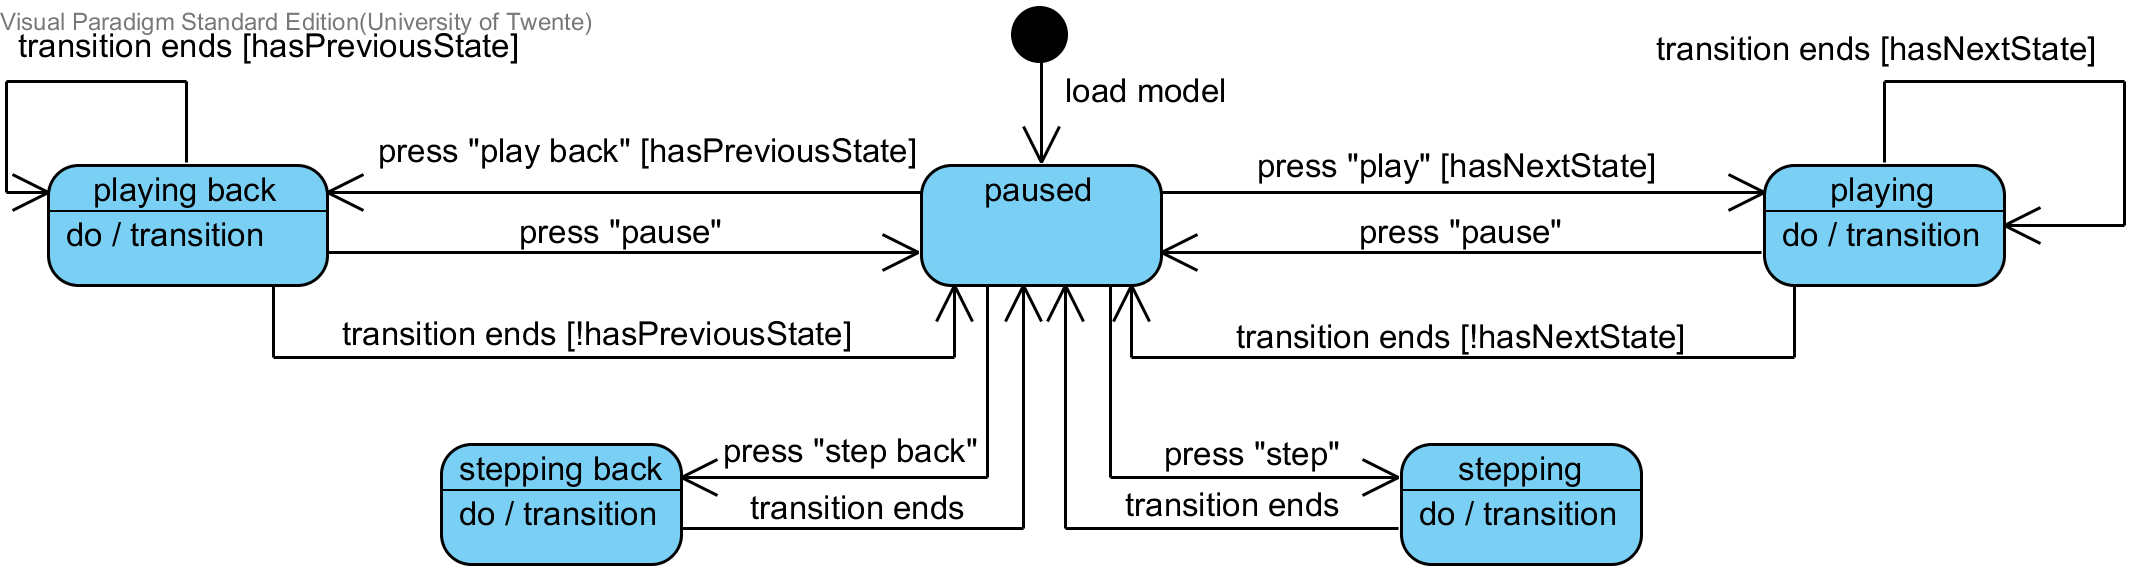
\includegraphics[width=\textwidth]{diagrams/smd_playbackstates}
  \caption{the state machine diagram for the visualizer's playback states}\label{fig:smd_playbackstates}
\end{figure}
%--------------------------------------------------------------------------------
\subsection{Internal representation of visual node properties}\label{sec:design;sub:fxwrapper}
The \lstinline{FxWrapper} class and its subclasses store and track the FX properties of GreenMirror nodes, as is explained in \cref{sec:features;sub:nodrel}. Using a wrapper instead of directly using a JavaFX node instance has the following reasons.
\begin{enumerate}
\item \lstinline{FxWrapper} provides general methods such as converting FX data into an object that can be shared between client and server, or changing general properties like the rotation and opacity of a JavaFX node.
\item The implementations of abstract methods of \lstinline{FxWrapper} used by GreenMirror might differ per type of JavaFX node. For example: the calculations of a specific placement on the edge of a circle differ from the calculations of a placement on the edge of a rectangle.
\item For the logic in the user's model and the proper creation of state-transitions on the server, properties have to be set and changed during the processing of state-transitions in the model without directly affecting the FX in the visualizer. As will be explained in \cref{sec:design;sub:states}, changing actual properties of JavaFX nodes happens as a consequence of the execution of JavaFX transitions. To work with these values without directly visualizing them, a wrapping layer is needed providing 'virtual' values. 
\item Support for new types of JavaFX nodes can be easily added. Examples include ellipses, three-dimensional shapes and composite nodes.
\end{enumerate}
The way \lstinline{FxWrapper} converts its properties to an object that can be sent over the network, is generalized in the sense that support for new types of properties can also be implemented easily. The following example will clarify this. One of the supported properties of \lstinline{ImageFxWrapper} is the X coordinate of type \lstinline{double}. In the current GreenMirror version, FX data is sent to the server in JSON format (see \cref{sec:design;sub:interchange}). The value of the X coordinate can be easily converted to and from a string format, as would the \lstinline{boolean}-type \lstinline{preserveRatio} property. So how would the \lstinline{image} property of type \lstinline{javafx.scene.image.Image} be converted to and from a valid JSON string? The implementations of \lstinline{FxPropertyWrapper} handle the FX properties to make this modular and easily extensible. In the case of the example about the image, the \lstinline{ImageFxProperty} class handles the \lstinline{image} property.
%--------------------------------------------------------------------------------
\subsection{Internal representation of states and state-transitions}\label{sec:design;sub:states}
\begin{wrapfigure}{o}{0.38\textwidth}\vspace{-20pt}
\begin{center}
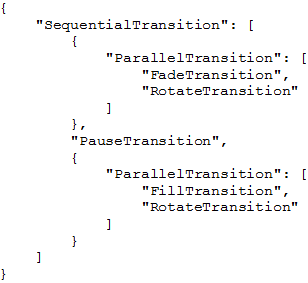
\includegraphics[width=0.36\textwidth]{diagrams/transitiontree}
\end{center}
\vspace{-10pt}\caption{an example of one stored state-transition in JSON notation}\vspace{-12pt}
\label{fig:transitiontree}
\end{wrapfigure}
State data is not stored in the current version of GreenMirror, because it is unnecessary. To understand why this is, an explanation must be provided about how state-transition data is stored and how JavaFX handles its transitions (animations, in this case).
\par GreenMirror uses classes that extend \lstinline{javafx.animation.Transition}. These classes hold all data needed to perform an animation: start and end value of an FX property and a method that handles the temporal behaviour of the value. JavaFX also provides two special transition implementations: \lstinline{ParallelTransition} and \lstinline{SequentialTransition}. These handle other transitions that are added to their lists in parallel or sequentially, respectively, and can be nested.
This is also how GreenMirror stores a state-transition: one \lstinline{SequentialTransition} instance holding one or multiple \lstinline{ParallelTransition} instances (separated by a \lstinline{PauseTransition} to incorporate an optional delay) which in turn hold the individual \lstinline{Transition} instances that animate the change in properties. Initially, every change in the model the server receives ends up in the same top-level \lstinline{ParallelTransition}. The user might want to show several sequential animations during one state-transition. For this scenario, the flush command has been implemented. This results in the server creating a new \lstinline{ParallelTransition} instance in the root \lstinline{SequentialTransition} in which all further transitions will be stored. For an example of these nested transitions of one state-transition, see \cref{fig:transitiontree}. JavaFX' transition classes also have another interesting functionality: the \lstinline{rate} property. When set to a negative value, the animation reverses. This makes browsing backwards through the model's states very easy and removes the need to recalculate FX property values of JavaFX nodes.
\par These reasons make storing state data unnecessary. State-transition data is composed of the JavaFX animations needed to go from one state to another, including the start and end values of the relevant FX properties, whichever direction the user wants to go.
%--------------------------------------------------------------------------------
\subsection{Interchange formats}\label{sec:design;sub:interchange}
Nothing is currently being stored of the result of a visualization. The formats associated with defining the user's model and the corresponding trace are discussed in \cref{sec:design;sub:interface}. This leaves the protocol used between the client and the server. This is very simple and has the form \texttt{command:commanddata}. The part before the colon holds the name of the command as it is presented in \cref{sec:features;sub:commands}. This is included so the receiver knows which \lstinline{CommandHandler} implementation can handle the command data. The part after the colon holds the command data, formatted in the selected \lstinline{CommunicationFormat}. The JSON format is currently the only supported format. An example of a command is shown in \cref{lst:commandexample}.
\begin{lstlisting}[label={lst:commandexample}, caption={an example command sent from the client to the server in the JSON communication format, indicating that a node as been added to the model}]
AddNode:{"id":2,"identifier":"nodetype:nodename"}
\end{lstlisting}
\newpage
%--------------------------------------------------------------------------------
%----------------------------------------------------------------------
\section{Validation}\label{sec:validation}
Unit tests have been written with the JUnit library that validate the classes the user works with the most: \lstinline{Node}, \lstinline{Relation}, \lstinline{NodeList}, \lstinline{RelationList}, \lstinline{FxWrapper}, \lstinline{FxWrapper}'s subclasses, \lstinline{Placement} and \lstinline{Placement}'s subclasses. The unit tests include the various ways of instantiating new objects, calling their methods with extreme values and in the case of the \lstinline{Placement} tests, they verify the calculations made to place a node in a certain respect to another node. These tests all worked as expected.
\par Due to the visual nature of GreenMirror, further verification is based on an extensive system test, written for use with the Groovy script model initializer. This test also works to some extent as a unit test: it tests several classes and specific functionalities. Furthermore, it showcases and explains how certain functionalities work and how they can be used. Among other sub-tests, it tests the following:
\begin{itemize}
\item setting the duration of animations;
\item using parameters from state-transition names;
\item adding nodes;
\item setting the FX of nodes;
\item altering the general properties of nodes;
\item altering properties specific for shape nodes (rectangle, circle and text nodes);
\item altering properties of a rectangle node;
\item altering properties of an image node;
\item altering properties of a text node;
\item adding and removing simple relations between nodes;
\item adding and replacing placement relations;
\item using rigid placement relations;
\item using chained, rigid placement relations; and
\item removing nodes.
\end{itemize}
\par A coverage of 84.8\% has been achieved with all tests combined. GreenMirror uses the \lstinline{@NonNull} annotation with fields and method arguments and return types. Not all sub-packages of Java formally guarantee that they return a non-null object (although they do informally), resulting in several non-null checks that are effectively futile and practically non-reachable code.
\par All test cases discussed in \cref{sec:intro;sub:project} have been successfully visualized. A screenshot of the results are illustrated in \cref{fig:greenmirror_ferryman,fig:connectfour,fig:phil}. They were all fairly easy to construct using the Groovy script model initializer. The realization of the ferryman case was a bit more elaborate compared to the realization discussed in \cref{sec:ferryman}, although the case itself and \cref{fig:greenmirror_ferryman} are essentially the same for both realizations. The test case, for example, also includes the state-transition where one cargo object 'eats' another. \Cref{tab:testcases} lists all relevant results of the three test cases.
\newpage\begin{longtable}{|l|r|r|r|p{6.7cm}|}
\caption{test case results}\label{tab:testcases}\\
\hline \textbf{Test case} 
     & \multicolumn{1}{|p{0.9cm}|}{\textbf{lines of code}}
     & \multicolumn{1}{|p{1.0cm}|}{\textbf{trace length}} 
     & \multicolumn{1}{|p{1.2cm}|}{\textbf{init. time}\footnote{Initialization time: the time GreenMirror needs to interpret the model and generate the visualizations.}} 
     & \textbf{notable visualizations and used functionalities} \\
\hline Ferryman            & 109 & 20 & $\approx$ 48 s & Parametrized state-transition names, rectangle FX types, image FX types, node resizing, node rotation, node removal, placement relations, rigid placement relations, non-placement relations, relation replacements, colour gradients \\
\hline ConnectFour         &  91 & 10 &  $\approx$~~8 s & Parametrized state-transition names, rectangle FX types, circle FX types, text FX types, node grid generated with \texttt{GridBuilder,} node creation during state-transition, colour gradients, font size setting, placement relations, relation replacements, complex model logic (determining the cell number from the column number), model failing (if an invalid move is encountered on the trace), altering animation duration \\
\hline Dining Philosophers & 132 & 15 & $\approx$ 10 s & Parametrized state-transition names, circle FX types, image FX types, image alteration during state-transition, node rotation, placement relations, non-placement relations, relation replacement, model failing (if an impossible state-transition is encountered) \\
\hline\end{longtable}
\begin{figure}[h]
\centering
    \begin{subfigure}[b]{0.53\textwidth}
    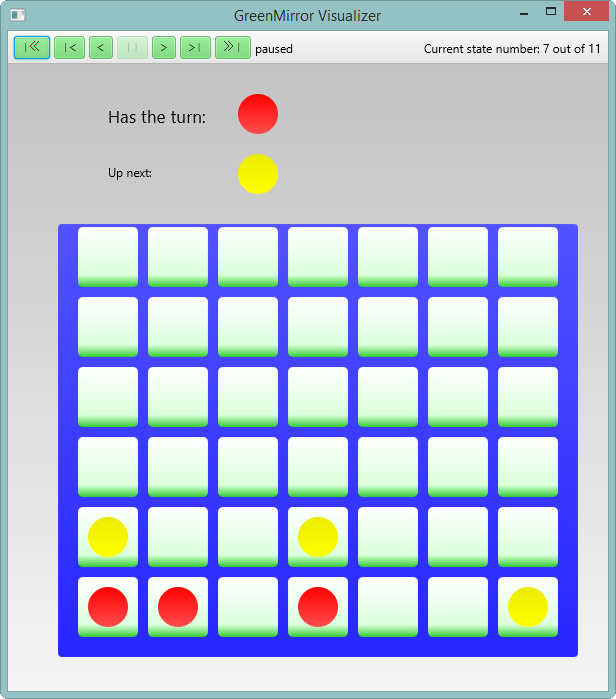
\includegraphics[width=\textwidth]{images/connectfour}
    \caption{ConnectFour}\label{fig:connectfour}
    \end{subfigure}
    ~
    \begin{subfigure}[b]{0.44\textwidth}
    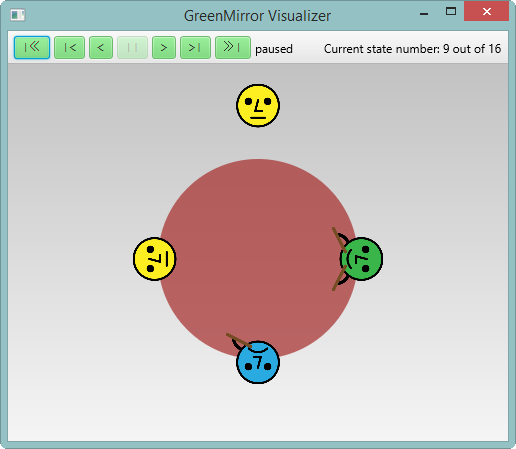
\includegraphics[width=\textwidth]{images/phil}
    \caption{Dining Philosophers}\label{fig:phil}
    \end{subfigure}
\caption{screenshots of two of the test cases}\label{fig:connectfour_phil}
\end{figure}
\par The following list discusses how each requirement and use case is implemented and validated, in the same order as they were defined in \cref{sec:intro;sub:project}.
\begin{description}
\item\textbf{\Cref{req:extensible,uc:extend}}\\The framework is easily extensible due to the use of interfaces and abstract classes. One example is the \lstinline{FxWrapper} class: support for new FX elements can be easily added by extending \lstinline{FxWrapper}. Also, the use of common design patterns makes extension more easy. See \cref{app:ext} for a full list of extensible parts.
\item\textbf{\Cref{req:maintainable}}\\The use of common design patterns, extensive documentation and the use of the checkstyle plugin of Eclipse are the primary means of making the framework maintainable. Especially the model-view-controller pattern is important because it tells which classes are responsible for what. More details on the design patterns can be found in \cref{sec:design;sub:patterns}.
\item\textbf{\Cref{req:aware_model,uc:model_aware,uc:model_source}}\\The application becomes aware of the user's model via the use of the model initializers: implementations of \lstinline{ModelInitializer}. It depends on the implementation how this is done. The choice of the implementation is how \cref{uc:model_aware} is supported: by use of the command line options and specifically the \lstinline{ModelCommandLineOptionHandler} class that handles the choice. This option handler accepts one argument: the source of the model (\cref{uc:model_source}) and it depends on the \lstinline{ModelInitializer} implementation how this source is given (for example: a file name or a model name).
\item\textbf{\Cref{req:aware_trace,uc:trace_source}}\\The user can pass his choice for the trace source via the command line and gets handled by the \lstinline{TraceCommandLineOptionHandler} class. The user's chosen \lstinline{TraceSelector} implementation then retrieves the trace and that is how the application becomes aware of the trace.
\item\textbf{\Cref{req:show_vis,req:show_vis_geom,req:show_vis_text,req:show_vis_imag,req:show_vis_anim,req:show_vis_plac,uc:vis}}\\A few examples of where the validation of these requirements is visible (as seen in \cref{fig:greenmirror_ferryman,fig:connectfour,fig:phil}): the ConnectFour test case visualizes rectangles, circles (\cref{req:show_vis_geom}) and text (\cref{req:show_vis_text}); the ferryman test case visualizes images (\cref{req:show_vis_imag}); and the dining philosophers test case visualizes the placement of nodes with respect to other nodes (\cref{req:show_vis_plac}). All test cases visualize simple animations (\cref{req:show_vis_anim}), which of course is not visible in the figures. The fact that these test cases can be visualized validates \cref{req:show_vis,uc:vis}.
\item\textbf{\Cref{req:log,uc:log}}\\This is implemented by the \lstinline{Log} class, as is discussed in \cref{sec:features;sub:log} and visible in \cref{fig:log} (page~\pageref{fig:log}).
\item\textbf{\Cref{req:browse,uc:browse}}\\Browsing from state to state is implemented by use of a toolbar with navigation buttons. The workings of these buttons are handled by the \lstinline{Visualizer} controller in cooperation with the \lstinline{PlaybackState} implementations and \lstinline{ToolbarButton} class. \Cref{sec:design;sub:patterns} discusses the playback state and its effect on the toolbar buttons. The buttons are also visible on any of the screenshots of GreenMirror in this report.
\item\textbf{\Cref{req:nodelay,req:nocrash}} \\Smoothly transitioning from state to state (\cref{req:nodelay}) is implemented by cleaning up resources every time the visualizer is closed. This 'resets' the server so a new client can connect. Crashing is prevented (\cref{req:nocrash}) by properly catching exceptions while the model is being loaded: this makes sure the visualizer will not crash during the state-transitions. If any exceptions are thrown, they will be displayed in the log.
\end{description}
\newpage
%--------------------------------------------------------------------------------
%----------------------------------------------------------------------
\section{Discussion}\label{sec:discussion}
GreenMirror is the second step in the development of an extensive research tool. The work of Aalbertsberg \cite{aalbertsberg2015} was the first step, although except for minor design choices such as the programming language and the client-server structure, his work bears virtually no resemblance to the current version. 

The intention for using a proper framework design was present during the design phase. Examples include the work of Fayad \& Schmidt \cite{fayad1997} and Markiewicz \& De Lucena \cite{markiewicz2001}, but this has crept unwittingly into the background during the implementation phase. Some concepts have been used (e.g. hot spots), but more research should be used while further developing the GreenMirror framework. A somewhat similar point applies to the use of the MVC pattern. It is implemented, as discussed in \cref{sec:design;sub:patterns}, but there is room for improvement to increase the framework's maintainability. For example: the distinction between the controller and view roles on the server side could be made more apparent and the view role on the client side could be improved beyond the use of just the \lstinline{Log} class.

Help from work relating to GreenMirror's way of visualization could not be uncovered. Due to the absence of related work backing the used visualization approach, this is a point of discussion. "Visualization approach" here means: the way of visualization (nodes and their FX representation) and the internal representation, which are discussed in \cref{sec:features;sub:nodrel,sec:design;sub:fxwrapper,sec:design;sub:states}. I believe the current approach is optimal for the requirements set for this project. It makes sure state-transitions can take place smoothly and without delay. It would probably, however, not be sufficiently efficient when GreenMirror is developed beyond the scope of this project. As is discussed in \cref{sec:validation}, it can take GreenMirror nearly a minute to convert a simple model to a visualization. That model had merely 20 state-transitions. Therefore, my first recommendation is to evaluate the current programmed structures and internal representations.

There is currently a \lstinline{TraceSelector} implementation in development by the Formal Methods and Tools research group of the University of Twente to select a trace from the GROOVE application. A next improvement to GreenMirror could be the development of a \lstinline{ModelInitializer} implementation that can load a model from an existing GROOVE Grammar. This would narrow the bridge between the two tools and would certainly be considered a useful functionality. The user might be required to provide extra information about how GROOVE’s nodes should be represented on the visualizer, should such an implementation be developed. Fortunately this can be done rather simple: the user can provide a script that uses the Groovy script model initializer to supplement the model, which is possible because the use of multiple model initializers is supported. 
%Additionally, a supplement to the Groovy script model initializer could be written that constructs a model in the format of another tool from the user's model. This would not be easy due to the different formats of different tools, but shouldn't be impossible. This way, a model could be analysed by defining it one time in stead of defining it for every tool used for analysis.
\\\\\par
To conclude this report, some thoughts must be given about the ultimate goal of this tool. In addition to generating visualizations from a defined model, the ultimate goal is, as is briefly mentioned in \cref{sec:intro;sub:project}, generating a model definition from of user interaction with visualizations.

Take a model where a state-transition results in the movement of a node from one location to another. A next extension of GreenMirror could allow the user to drag a node in the visualizer from one location to another. Assuming both location boundaries have been properly defined, the application can recognize this as a state-transition. In this scenario the user can alter the trace, adding state-transitions before, in-between or after the transitions on the original trace.

There are of course many more visualization possibilities than simply moving a node. Continuing and expanding on the previous scenario: in stead of the atomic interaction of dragging a node to another location, the user could record multiple changes in the visualizer, resulting in a new state-transition definition or in the recognition of a previously defined state-transition. This might work fine solely for recognizing state-transitions, but this still has considerable limitations in the creation of new state-transitions.

The next step is the addition of the creation of model logic. In the GreenMirror application, a transition in the model could be defined as such: "if node A and node B both have a relation with node C, remove the relation between node A and node C and add a new relation between node A and node D". In this step of the development of this extension, a user should be able to create such logic based on his interactions with the visualizer. This can become complex very fast, but that should be considered an interesting challenge to accept in the future.

The next and perhaps final step is to make a two-way connection with other tools that enable or facilitate the research of state-transition models in different ways. When the connection is made between interactions with the visualizer and the creation of state-transition logic, this could be translated into a format that can be accepted by other tools. This way, the need is eliminated for researchers to rewrite their models into tool-specific formats when different tools are used.



\bibliography{bibliography}
\newpage
\appendix
%--------------------------------------------------------------------------------
%----------------------------------------------------------------------
\section{Service extension instructions}\label{app:ext}
This appendix gives instructions on how to extend several components of the GreenMirror framework. These components have been specifically designed to be easily extensible with as few steps as possible. The final, omitted step after adding an extension is to recompile, so the extension can be used. This section is meant for developers, although \cref{app:ext;sub:modelinitializer,app:ext;sub:traceselector} are mainly meant for tool owners. Both of these stakeholder groups are assumed to have sufficient understanding of the Java programming language to comprehend these instructions. Most extensible components make use of the \lstinline{java.util.ServiceLoader} injector. More in-depth details about implementing new code is available in the JavaDocs on the repository of this project.
%--------------------------------------------------------------------------------
\subsection{\texttt{ModelInitializer}}\label{app:ext;sub:modelinitializer}
\begin{enumerate}
  \item Implement \lstinline{greenmirror.client.ModelInitializer}, making sure that it has a zero-argument constructor.
  \item Add the fully-qualified binary class name of your new class with a new line to the file \lstinline{META-INF/services/greenmirror.client.ModelInitializer}.
\end{enumerate}
%--------------------------------------------------------------------------------
\subsection{\texttt{TraceSelector}}\label{app:ext;sub:traceselector}
\begin{enumerate}
  \item Implement \lstinline{greenmirror.client.TraceSelector}, making sure that it has a zero-argument constructor.
  \item Add the fully-qualified binary class name of your new class with a new line to the file \lstinline{META-INF/services/greenmirror.client.TraceSelector}.
\end{enumerate}
%--------------------------------------------------------------------------------
\subsection{\texttt{FxWrapper}}\label{app:ext;sub:fxwrapper}
\begin{enumerate}
  \item Extend \lstinline{greenmirror.FxWrapper} or \lstinline{greenmirror.FxShapeWrapper} if the JavaFX node type your new class is representing is an extension of \lstinline{javafx.scene.shape.Shape}. In either case make sure that it has a zero-argument constructor.
  \item Add the JavaFX node properties you want to support (see \cref{app:ext;sub:fxpropertywrapper}).
  \item Add the fully-qualified binary class name of your new class with a new line to the file \lstinline{META-INF/services/greenmirror.FxWrapper}.
\end{enumerate}
%--------------------------------------------------------------------------------
\subsection{\texttt{FxPropertyWrapper}}\label{app:ext;sub:fxpropertywrapper}
\begin{enumerate}
  \item Extend \lstinline{greenmirror.FxPropertyWrapper}.
  \item Support for this FX property type is being added to support a specific FX property of an \lstinline{FxWrapper} subclass. An entry must be added to one of two methods of the relevant \lstinline{FxWrapper} subclass. If the FX property can be animated, add an entry to the \lstinline{getAnimatableProperties()} method. If the property can only be set once, add it to the \lstinline{getChangableProperties()} method.
  \item Add one or more get-methods to the \lstinline{FxWrapper} subclass.
  \item Add one or more set-methods to the \lstinline{FxWrapper} subclass. The type of the argument of the primary set-method depends on what the relevant \lstinline{FxPropertyWrapper}'s \lstinline{getPropertyType()} method returns.
  \item If the property can be animated, but hasn't got a \lstinline{javafx.animate.Transition} implementation yet, create it. The abstract \lstinline{AbstractTransition} and \lstinline{DoublePropertyTransition} classes have been created to provide several often used methods when extending \lstinline{javafx.animate.Transition}.
  \item If the property can be animated, add the animate method that returns the \lstinline{javafx.animate.Transition} that changes the value of the property when played.
  \item If the user needs access to the new property type in the Groovy model initializer, add an entry to the \lstinline{IMPORTS} constant of the \lstinline{greenmirror.client.modelinitializers.GroovyScriptModelInitializer} class.
\end{enumerate}
%--------------------------------------------------------------------------------
\subsection{\texttt{Placement}}\label{app:ext;sub:placement}
\begin{enumerate}
  \item Extend \lstinline{greenmirror.Placement}, making sure that it has a zero-argument constructor.
  \item If the placement has no further parameters (such as the angle parameter of \lstinline{EdgePlacement}), add a public constant to \lstinline{greenmirror.Placement} holding an instance of your new class.
  \item Add support for the new placement by adding the necessary calculations to the \lstinline{calculatePoint(Placement)} methods of all implemented \lstinline{FxWrapper}s and to the static \lstinline{calculatePointOnRectangle(double, double, Placement)} method of the \lstinline{FxWrapper} class. 
  \item Add the fully-qualified binary class name of your new class with a new line to the file \lstinline{META-INF/services/greenmirror.Placement}.
\end{enumerate}
%--------------------------------------------------------------------------------
\subsection{\texttt{Command}}\label{app:ext;sub:command}
\begin{enumerate}
  \item Extend \lstinline{greenmirror.Command}.
  \item Add a corresponding \lstinline{CommandHandler}. See \cref{app:ext;sub:commandhandler}.
\end{enumerate}
%--------------------------------------------------------------------------------
\subsection{\texttt{CommandHandler}}\label{app:ext;sub:commandhandler}
\begin{enumerate}
  \item Extend \lstinline{greenmirror.CommandHandler}, making sure that it has a zero-argument constructor and that its \lstinline{getCommand()} method returns the same string as the \lstinline{Command} class that this handler is meant to handle.
  \item Add at least one of the \lstinline{@ClientSide} and \lstinline{@ServerSide} annotations, indicating on which "side" the command should be handled.
  \item Add the fully-qualified binary class name of your new class with a new line to the file \lstinline{META-INF/services/greenmirror.CommandHandler}.
\end{enumerate}
%--------------------------------------------------------------------------------
\subsection{\texttt{CommandLineOptionHandler}}\label{app:ext;sub:cloh}
\begin{enumerate}
  \item Implement \lstinline{greenmirror.CommandLineOptionHandler}, making sure that it has a zero-argument constructor.
  \item Add at least one of the \lstinline{@ClientSide} and \lstinline{@ServerSide} annotations, indicating on which "side" the command line option should become available.
  \item Add the fully-qualified binary class name of your new class with a new line to the file \lstinline{META-INF/services/greenmirror.CommandLineOptionHandler}.
\end{enumerate}
%--------------------------------------------------------------------------------
\subsection{\texttt{Log}}\label{app:ext;sub:log}
\begin{enumerate}
  \item Extend \lstinline{java.io.PrintStream}.
  \item Add a \lstinline{Log.addOutput(instance);} statement to the entry point of the component you want to add it to. The entry point of the client is the static \lstinline{main(String[])} method of the \lstinline{greenmirror.client.Client} class. The entry point of the server is the \lstinline{start(Stage)} method of the \lstinline{greenmirror.server.Visualizer} class.
\end{enumerate}
\newpage
\section{Sequence diagrams}\label{app:seq}
All diagrams are simplified in the sense that they do not show every atomic operation and that they show only validation and error handling when it is relevant and essential to the understanding of the sequences. They are simplified to improve the overall orderliness and comprehensibility of the diagrams.
\begin{figure}[hb]
  \centering
  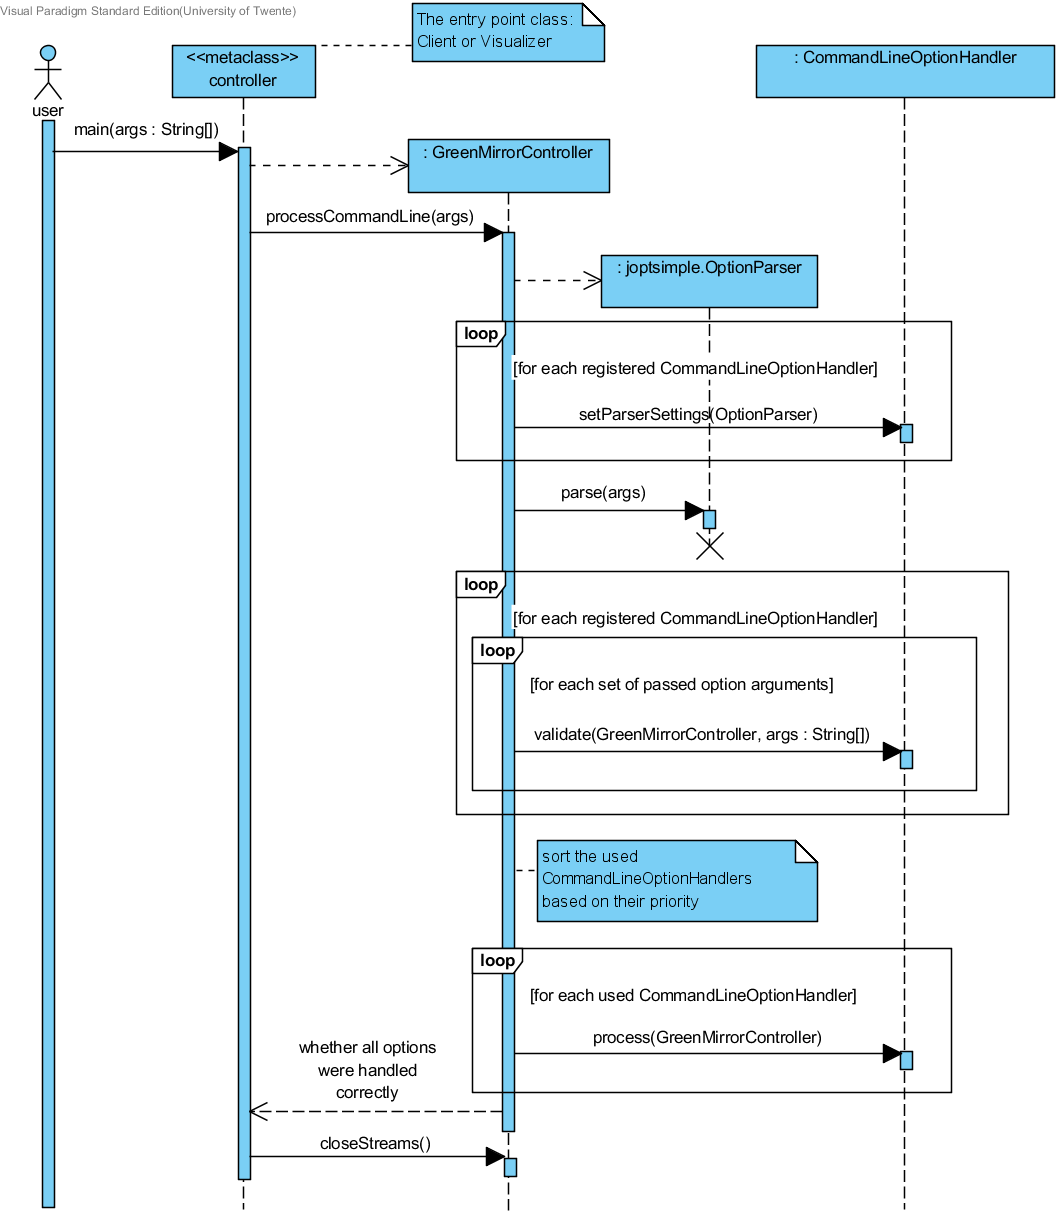
\includegraphics[width=0.96\textwidth]{diagrams/SD_generalstartup}
  \caption{simplified sequence diagram of the general start-up. There is a slight difference on the server side: if the options are all handled correctly, the controller doesn't close the streams, but starts listening for incoming connections.}\label{fig:sd_generalstartup}
\end{figure}
\begin{figure}[ht]
  \centering
  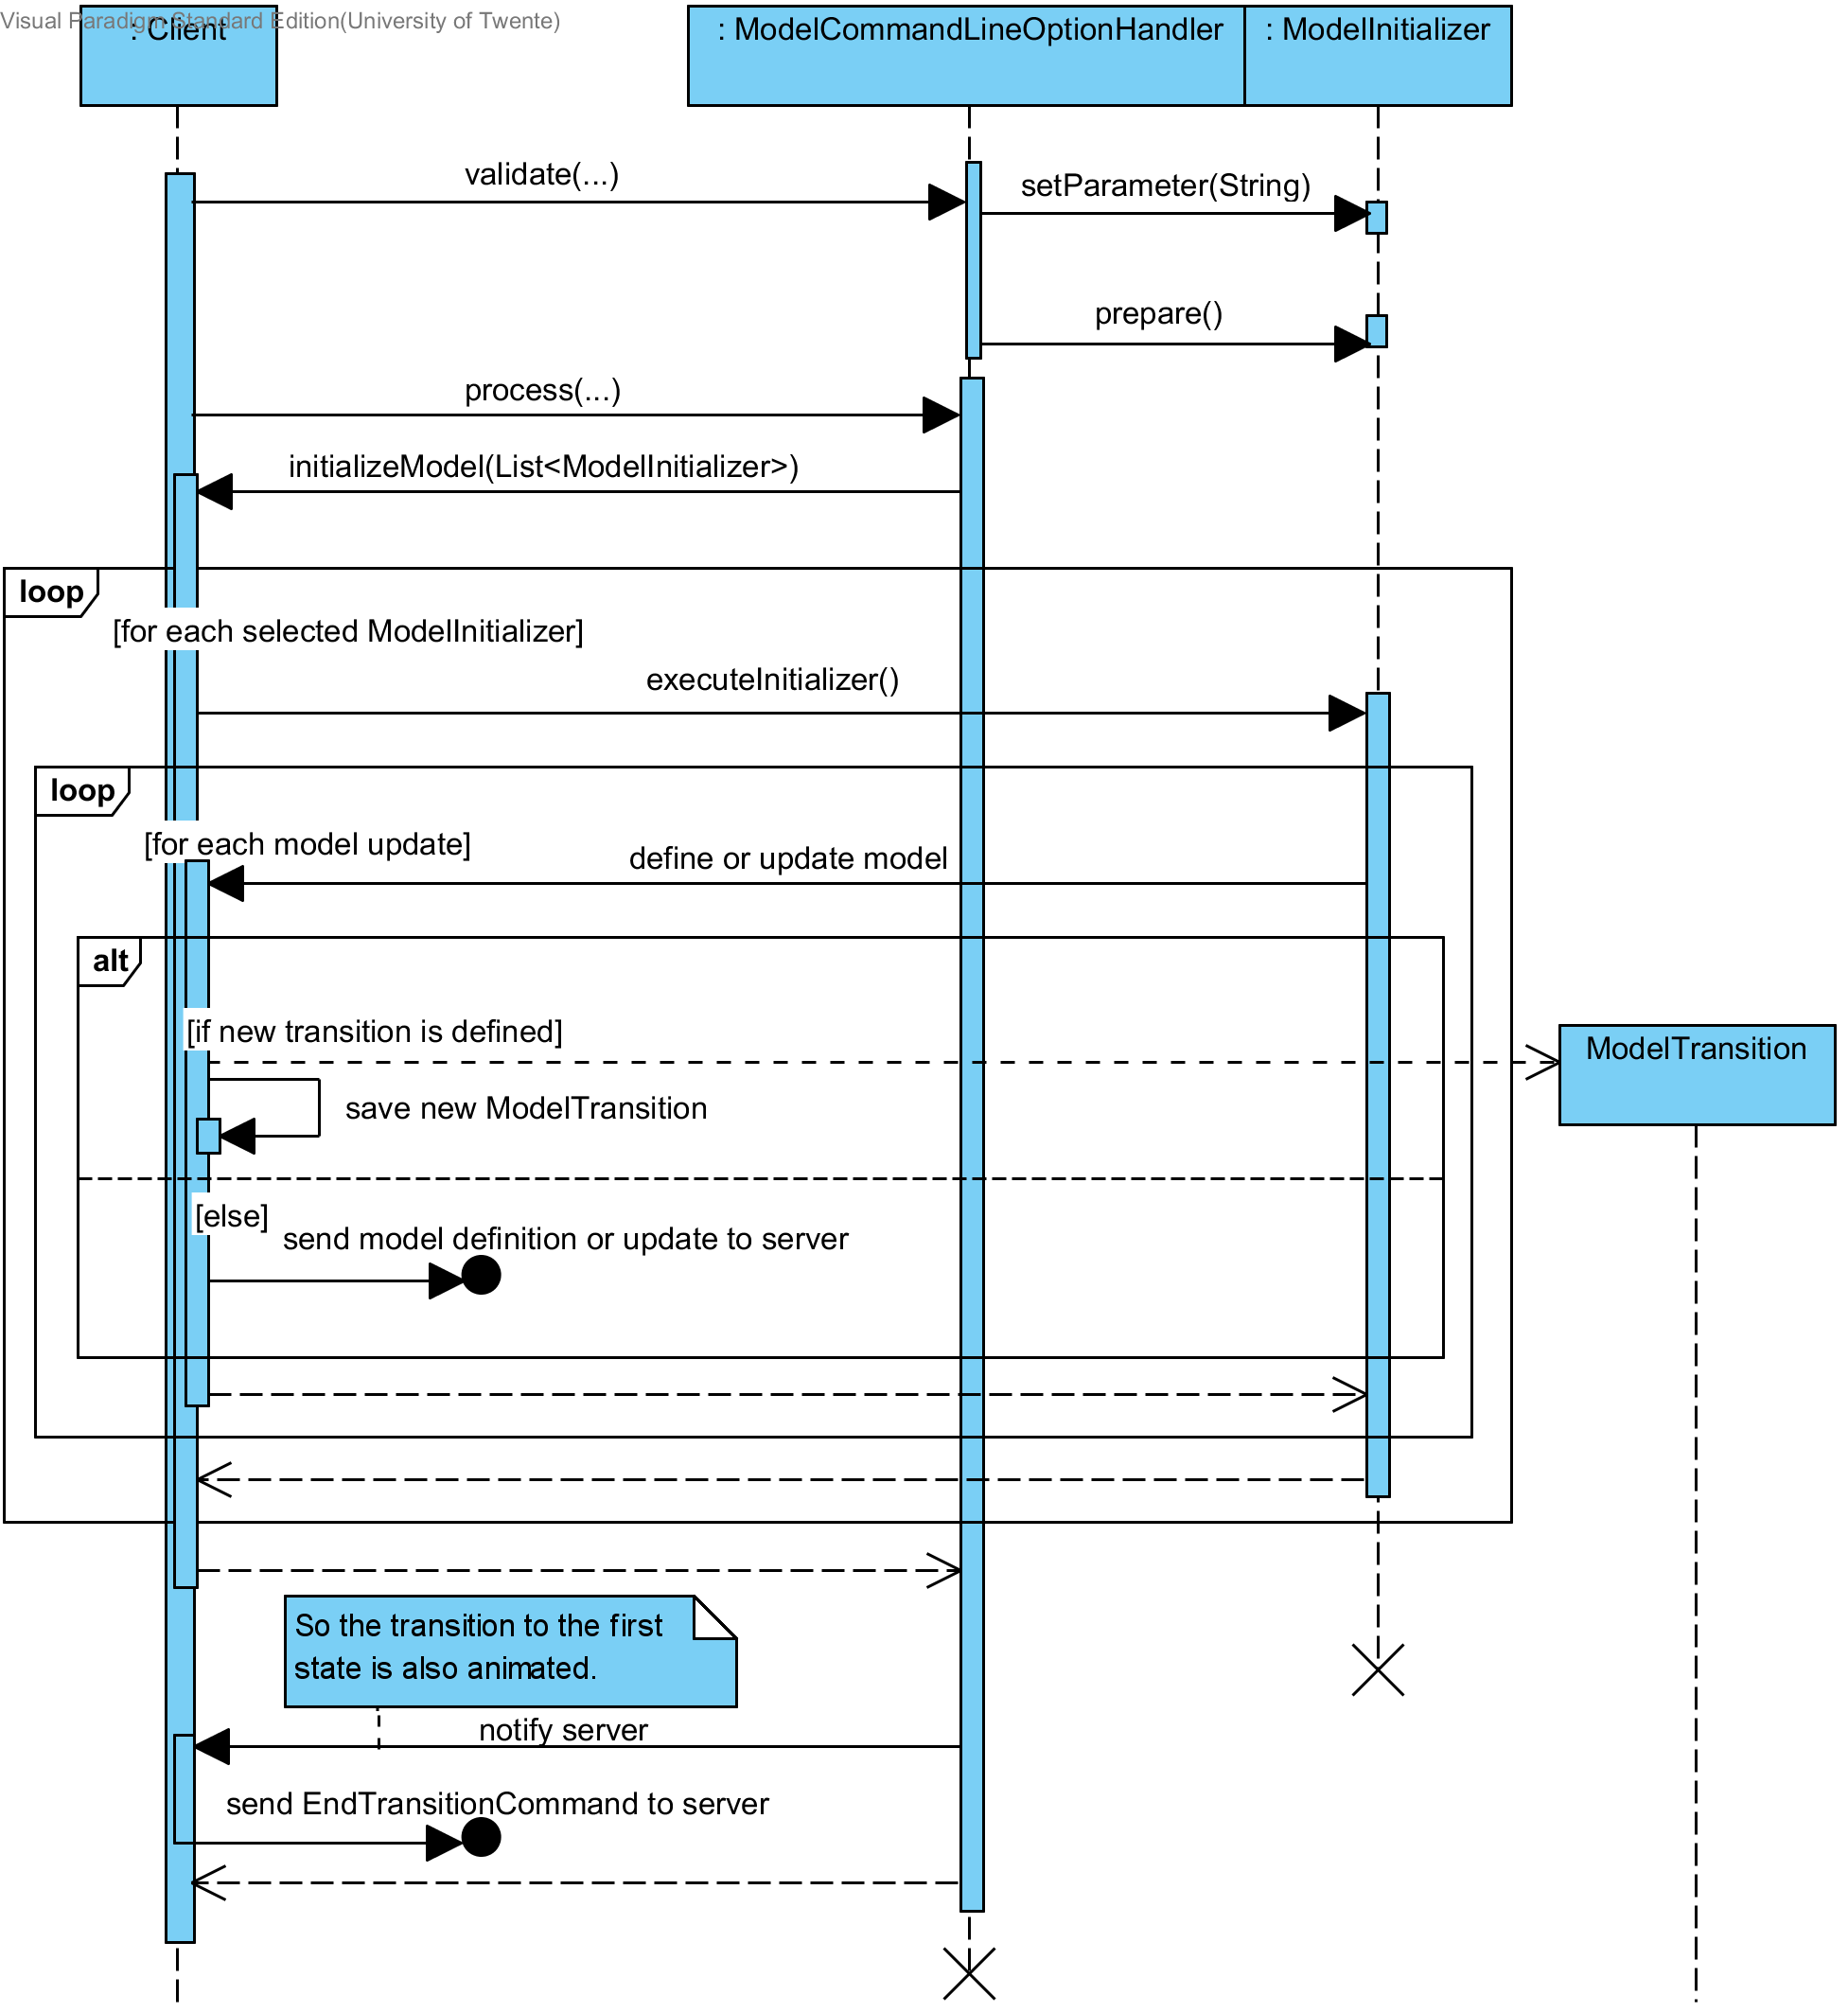
\includegraphics[width=1.1\textwidth]{diagrams/SD_client_model}
  \caption{simplified sequence diagram of the handling of the \lstinline{--model} command line option}\label{fig:sd_client_model}
\end{figure}
\begin{figure}[ht]
  \centering
  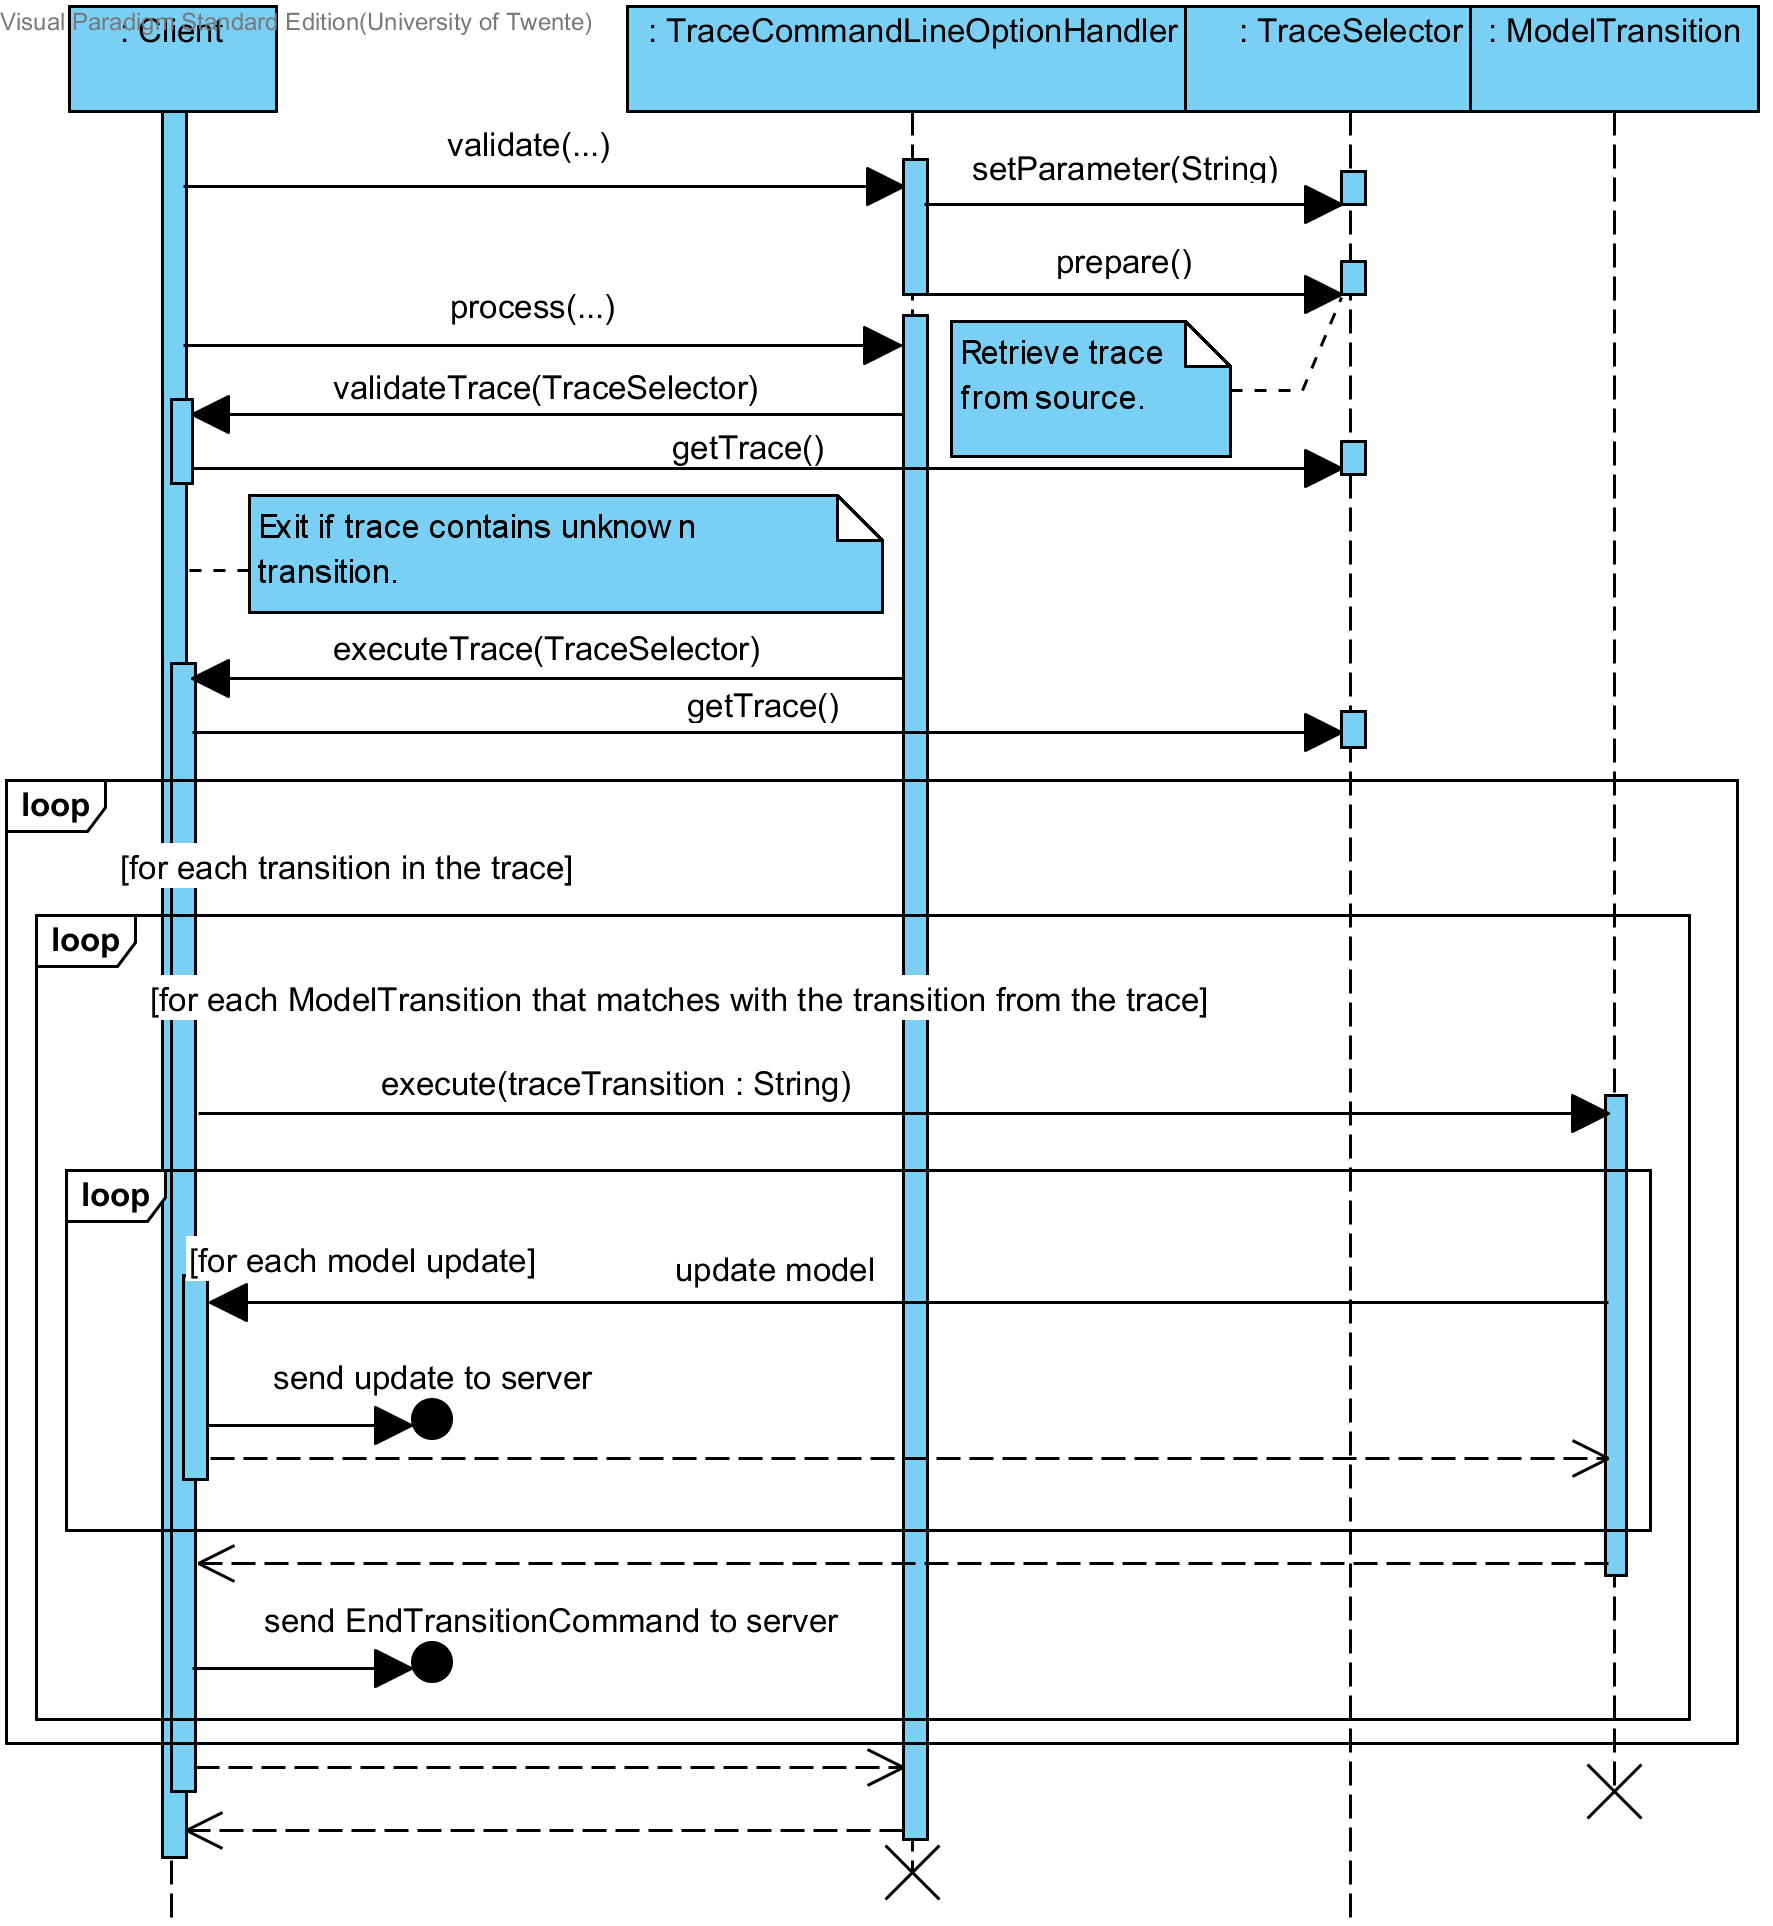
\includegraphics[width=1.1\textwidth]{diagrams/SD_client_trace}
  \caption{simplified sequence diagram of the handling of the \lstinline{--trace} command line option}\label{fig:sd_client_trace}
\end{figure}
\begin{figure}[ht]
  \centering
  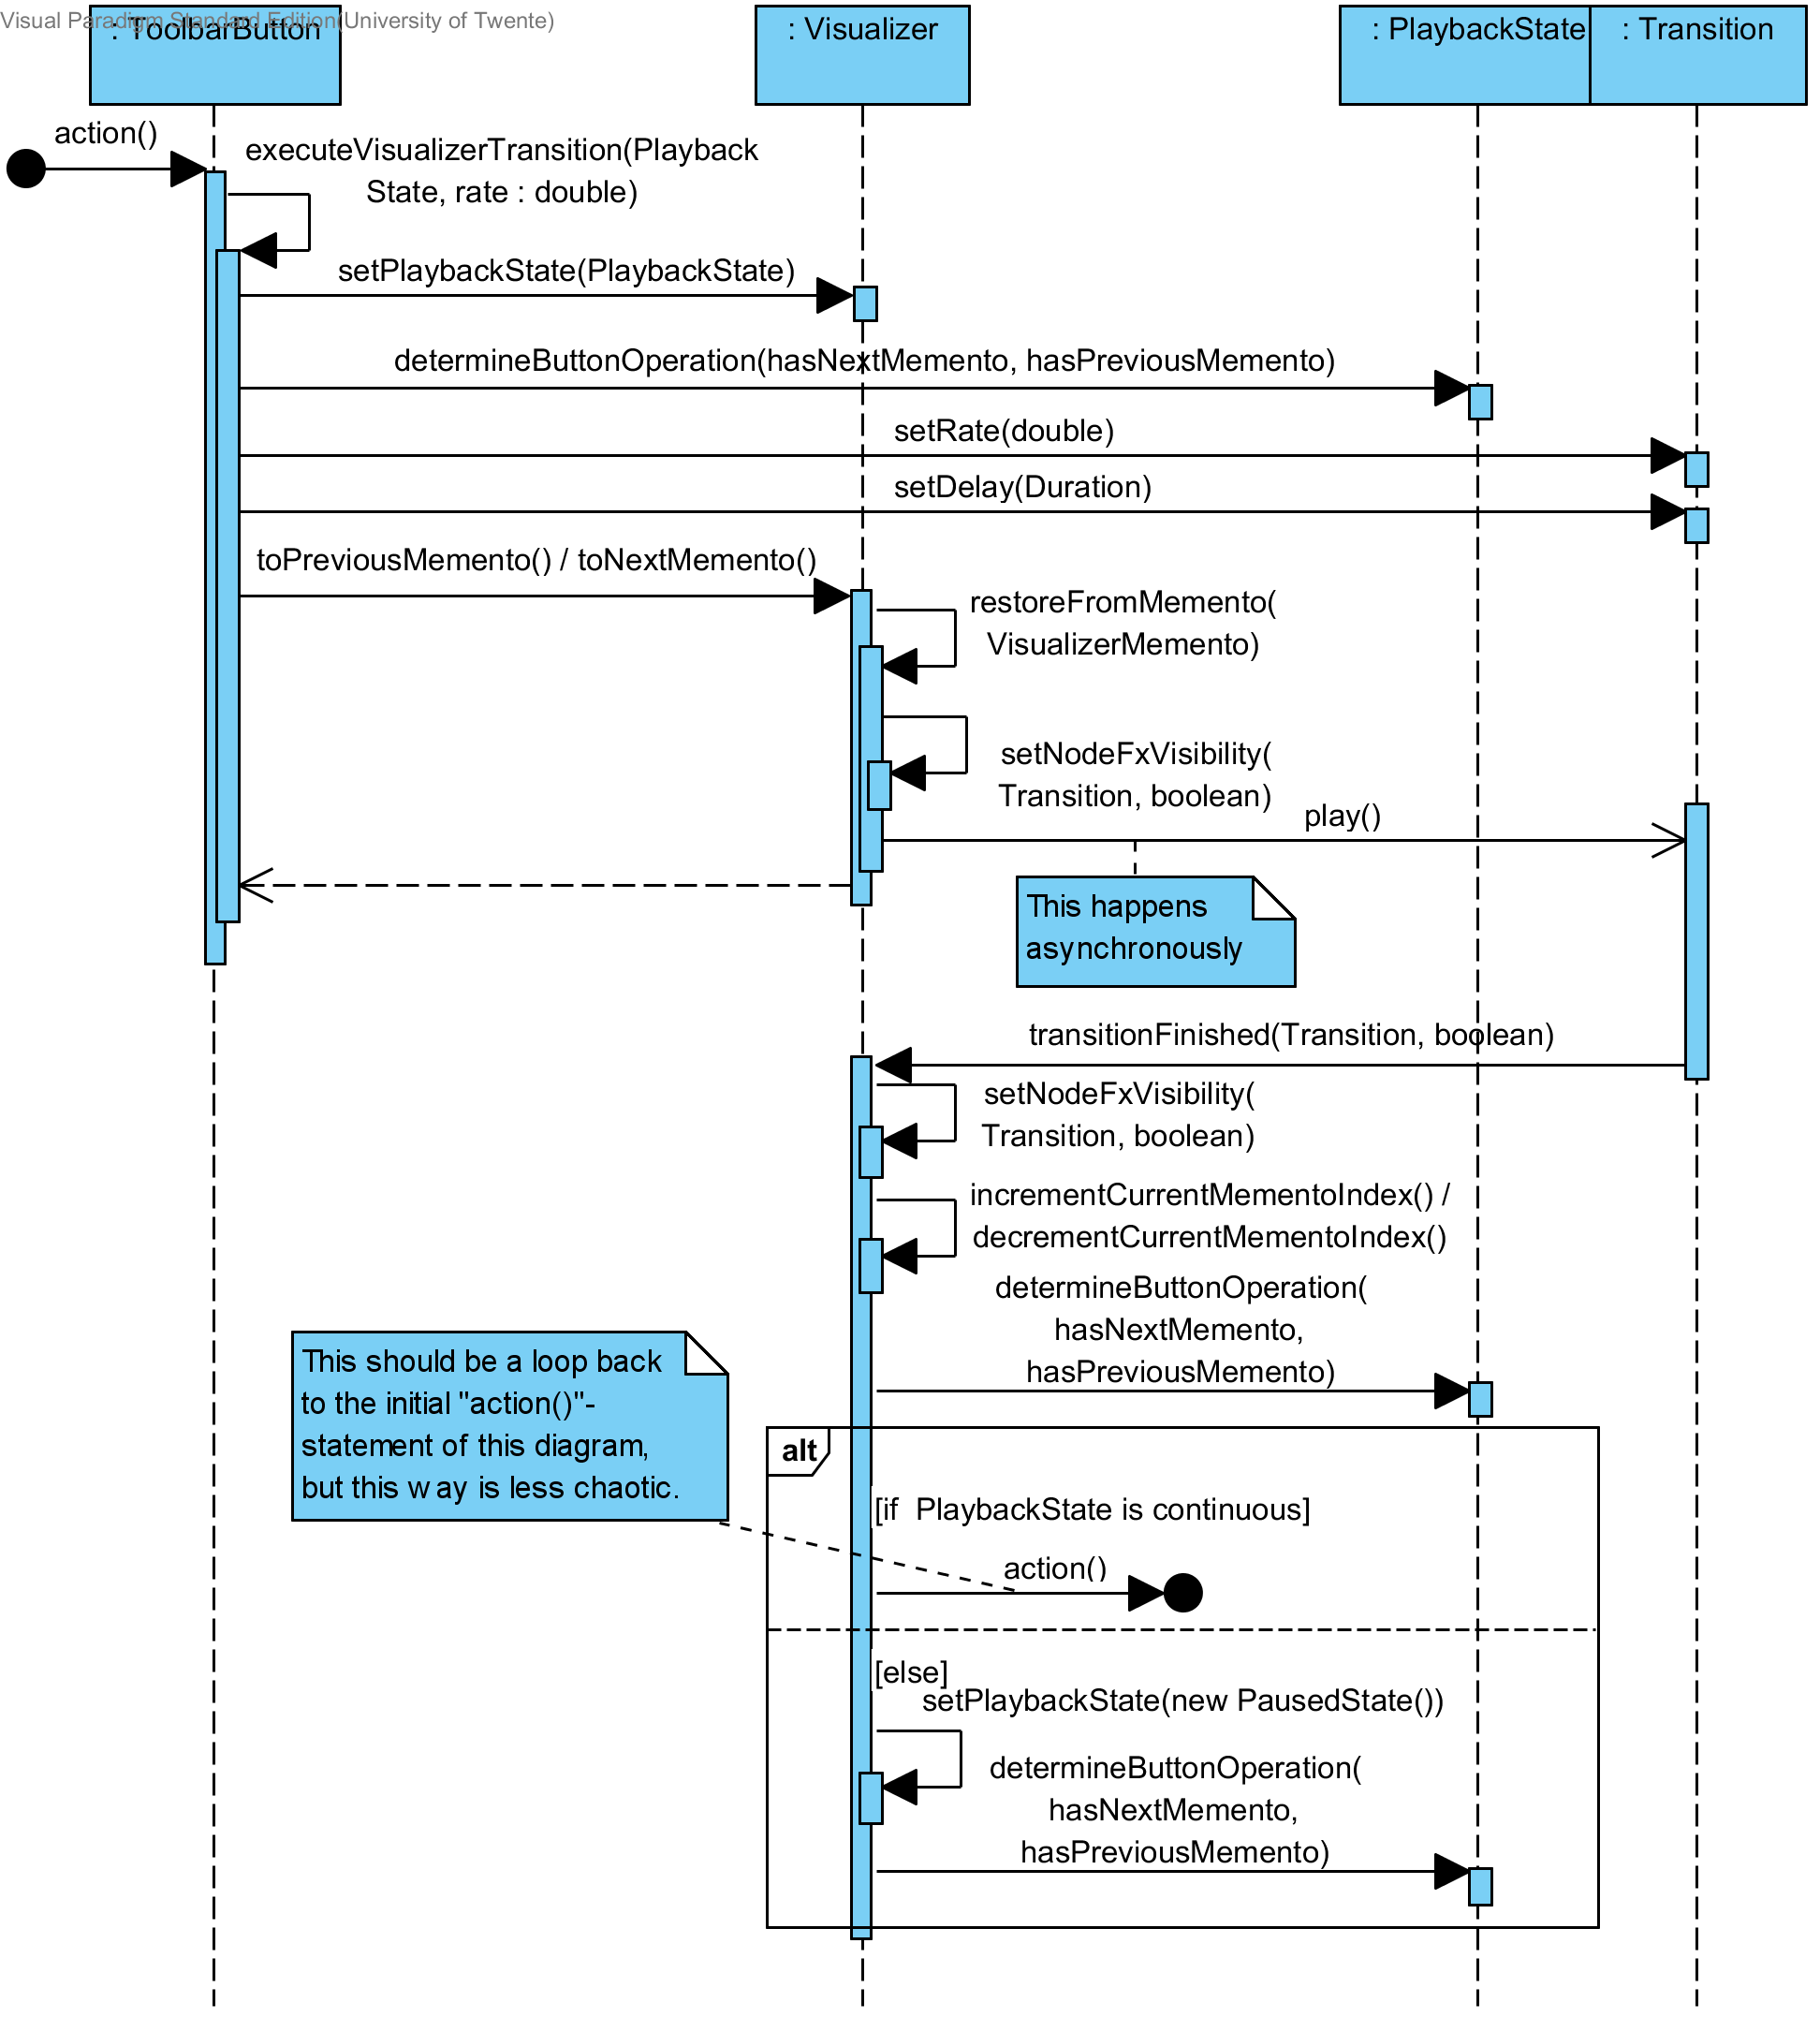
\includegraphics[width=1.1\textwidth]{diagrams/SD_server_userinteraction}
  \caption{simplified sequence diagram of user interaction with any one of the toolbar buttons (but not with the pause button)}\label{fig:sd_server_userinteraction}
\end{figure}

\end{document}